\chapter{Results}
\label{ch: results}

Floods can affect both supply and demand in the economy, making the overall impact on the outcomes of establishments uncertain. Disruptions to supply and infrastructure can increase costs for firms and encourage them to raise their prices or layoff workers. At the same time, job losses and lower household incomes, coupled with greater uncertainty, can depress demand. Turning to the effects on real economic activity in more detail, the impact of floods can vary greatly across sectors and regions. This section focuses on the impact of flooding measured on establishments outcomes and subsequently on those outcomes aggregated at the commune level.

\section{The impact of flooding on firms and workers}

Figure~\ref{fig:firms_results} plots the impulse response functions following a \textit{CatNat} flood for two key outcomes—wages and headcount—measured at the end of the year (31.12). As shown, the estimated leads ($k < 0$) are uniformly insignificant, supporting the parallel-trends assumption, while the lags ($k \geq 0$) reveal significant and persistent losses. Scaling the average post-treatment coefficients in Table~\ref{tab:lpdid_pooled} by the sample means in Table~\ref{tab:summary_stats} indicates that the estimated wage effect of –233.6 corresponds to a reduction of roughly $–1.1\%$ in 31.12 wages, while the employment effect of –0.15 workers translates into a decline of about $–1.7\%$ in 31.12 headcount. Since yearly averages (Figures \ref{fig:avg_wage_firm} and \ref{fig:avg_eff_firm}) do not display such pronounced movements, I interpret this as evidence of substantial rigidity in both wage-setting and layoffs in the French formal sector. One possible explanation is the strong enforcement of collective agreements by trade unions and employer associations.

It is instructive to compare these findings to other wage shocks in the literature—for example, those related to plant closures or mass layoffs. Such benchmarking would help assess whether floods generate disruptions of a similar scale, or whether wages respond differently to natural disasters. This comparison could also shed light on whether the labor market views climate-related shocks as primarily transitory or as persistent disruptions. The full set of coefficients underlying Figures \ref{fig:wage3112_firm} and \ref{fig:eff3112_firm} can be found in Table~\ref{tab:stacked_es_employment_wages}, while additional event-study graphs for other outcomes are shown in Figure~\ref{fig:firms_extra_results}.

Turning to contract composition, I do not find statistically significant changes in the share of permanent (CDI) versus temporary (CDD) contracts, although there is a modest but insignificant decline in CDD employment. This is consistent with the idea that end-of-year employment falls mainly because temporary workers are more easily dismissed than permanent staff, even if average yearly employment remains relatively stable. Furthermore, floods do not appear to reduce worker efficiency: hourly wages, a proxy for productivity per hour, remain broadly unchanged. Instead, the adjustment occurs through employment. However, the precise nature of this adjustment differs across measures. End-of-year headcount shows clear reductions, suggesting that separations take place around December 31, most likely through non-renewal of temporary contracts. By contrast, FTEs and turnover—which aggregate over the whole year—show little movement, indicating that these separations are concentrated in timing rather than reflecting sustained declines in labor input across the year. In other words, floods reduce employment at specific moments (the end of the year), but not enough to generate lasting losses in annual labor input or output.

The absence of clear effects on financial variables is also noteworthy. One explanation may be data limitations: monthly information on revenues and investments would be required to capture short-term disruptions, compensating capital expenditures, or capital retirement following floods. In addition, value added is not a clean measure of productivity, since it is endogenous to firms’ pricing and input allocation decisions; a cost-function approach would be needed to recover total factor productivity (TFP). Finally, there is an economic rationale for why labor adjusts more quickly than output or profit: floods immediately disrupt commuting, staffing, and local services, while revenues and profits may be temporarily cushioned by insurance payouts, government relief, or demand shifts (e.g. replacement purchases).
\vspace{0.5cm}


%\begin{table}[htbp]\centering
\caption{\textbf{Table \ref{tab:lpdid_pooled}}: Local-Projection DiD — Pooled Coefficients}
\label{tab:lpdid_pooled}
\renewcommand{\arraystretch}{1.1}
\begin{tabular}{l*{3}{c}}
\toprule
               &\multicolumn{1}{c}{(1)}&\multicolumn{1}{c}{(2)}&\multicolumn{1}{c}{(3)}\\
               &  \textbf{Employment}  &  Wages  &  CDI \\[-0.3em]
               &  \footnotesize{Total headcount at 31.12} & \footnotesize{Average wage at 31.12} & \footnotesize{Share of permanent contracts} \\ 
\midrule
\textit{Pre} coefficient      &  \num{0.0109}     & \num{-167.9653}\sym{***} & \num{0.0016} \\
                              &  (0.0300)         & (39.3618)                 & (0.0013)     \\
\textit{Post} coefficient     &  \num{-0.1497}\sym{**} & \num{-233.6222}\sym{***} & \num{0.0055}\sym{**} \\
                              &  (0.0629)         & (77.5715)                 & (0.0026)     \\[0.4em]
Observations                  &  396{,}994        & 357{,}851                 & 394{,}378    \\
\midrule
Commune fixed effects         & \checkmark & \checkmark & \checkmark \\
Year fixed effects            & \checkmark & \checkmark \checkmark \\
Département $\times$ Year FE  & \checkmark & \checkmark & \checkmark \\
Flood-history controls        & \checkmark & \checkmark & \checkmark \\
\bottomrule
\multicolumn{4}{p{12cm}}{\footnotesize
\textit{Notes:} Each column reports pooled LP-DiD “Pre” (mean of $k=-5\dots-2$) and “Post” (mean of $k=0\dots5$) coefficients.  
Robust standard errors clustered at the commune (\texttt{INSEE\_COM}) level in parentheses.  
\sym{*} $p<0.10$, \sym{**} $p<0.05$, \sym{***} $p<0.01$.}
\end{tabular}
\end{table}
%\begin{table}[!htbp]
\centering
\caption{\textbf{Table \ref{tab:lpdid_pooled}}: Local-Projection DiD — Pooled Post-Treatment Effects}
\label{tab:lpdid_pooled}
\renewcommand{\arraystretch}{1.1}
\resizebox{15.5cm}{!}{
\begin{tabular}{lccccc}
\toprule
& \textbf{EFF\_3112} & \textbf{AVGWAGE\_3112} & \textbf{CDD Share} & \textbf{EFF\_MOY\_ET} & \textbf{HWAGE} \\[-0.3em]
& \footnotesize{Employment in 3112 firms} & \footnotesize{Average wage in 3112 firms} & \footnotesize{Fixed-term contract share} & \footnotesize{Average establishment size} & \footnotesize{Hourly wage} \\
\midrule

\textit{Post-treatment effect} & $-$0.150\sym{**} & $-$233.62\sym{***} & $-$0.0026 & $-$0.4248 & $-$0.231\sym{**} \\
                               & (0.063) & (77.57) & (0.0025) & (0.2867) & (0.098) \\[0.5em]

\textit{Mono-establishment} (=1) & $-$0.022 & $-$524.13\sym{***} & $-$0.0052 & $-$0.0070 & $-$0.231\sym{**} \\
                                 & (0.020) & (127.62) & (0.0047) & (0.0229) & (0.098) \\[0.5em]

\textit{Litorale} (=1) & [TBD] & [TBD] & [TBD] & [TBD] & [TBD] \\
                       &       &       &       &       &       \\

\midrule
Observations (total)           & 6.82M & 6.82M & 6.82M & 6.82M & 6.82M \\
Commune fixed effects          & \checkmark & \checkmark & \checkmark & \checkmark & \checkmark \\
Year fixed effects             & \checkmark & \checkmark & \checkmark & \checkmark & \checkmark \\
Flood risk group fixed effects & \checkmark & \checkmark & \checkmark & \checkmark & \checkmark \\
Flood risk $\times$ Section $\times$ Year FE & \checkmark & \checkmark & \checkmark & \checkmark & \checkmark \\
Clustered SEs at commune level & \checkmark & \checkmark & \checkmark & \checkmark & \checkmark \\
\bottomrule
\multicolumn{6}{p{18cm}}{\footnotesize \textit{Notes:} Each column reports pooled LP-DiD estimates (average of event times $k = 0$ to $5$). Robust standard errors clustered at the commune level (\texttt{INSEE\_COM}) are reported in parentheses. $^{*}p<0.10$; $^{**}p<0.05$; $^{***}p<0.01$.}
\end{tabular}}
\end{table}




%The reduction in effective employment (FTE) by around 2\% is also notable and suggests real labor adjustments at the intensive margin. This aligns with the view that floods can interfere with daily operations, reduce hours, or temporarily suspend business activity, especially in local service sectors.


%%%%%%%%%%%%%%%%%%%%%%%%%%%%%%%%%%%%%%%%%%%%%%%%%%%%%%%%%
%%%%%%%%%%%%%%%%%%%%%%%%%%%%%%%%%%%%%%%%%%%%%%%%%%%%%%%%%
\begin{figure}[htbp]
  \centering

  \caption{\textbf{Figure \ref{fig:firms_results}:} Impact of floods on firms outcomes}
  \label{fig:firms_results}
  
  \begin{subfigure}[t]{0.49\textwidth}
    \centering
    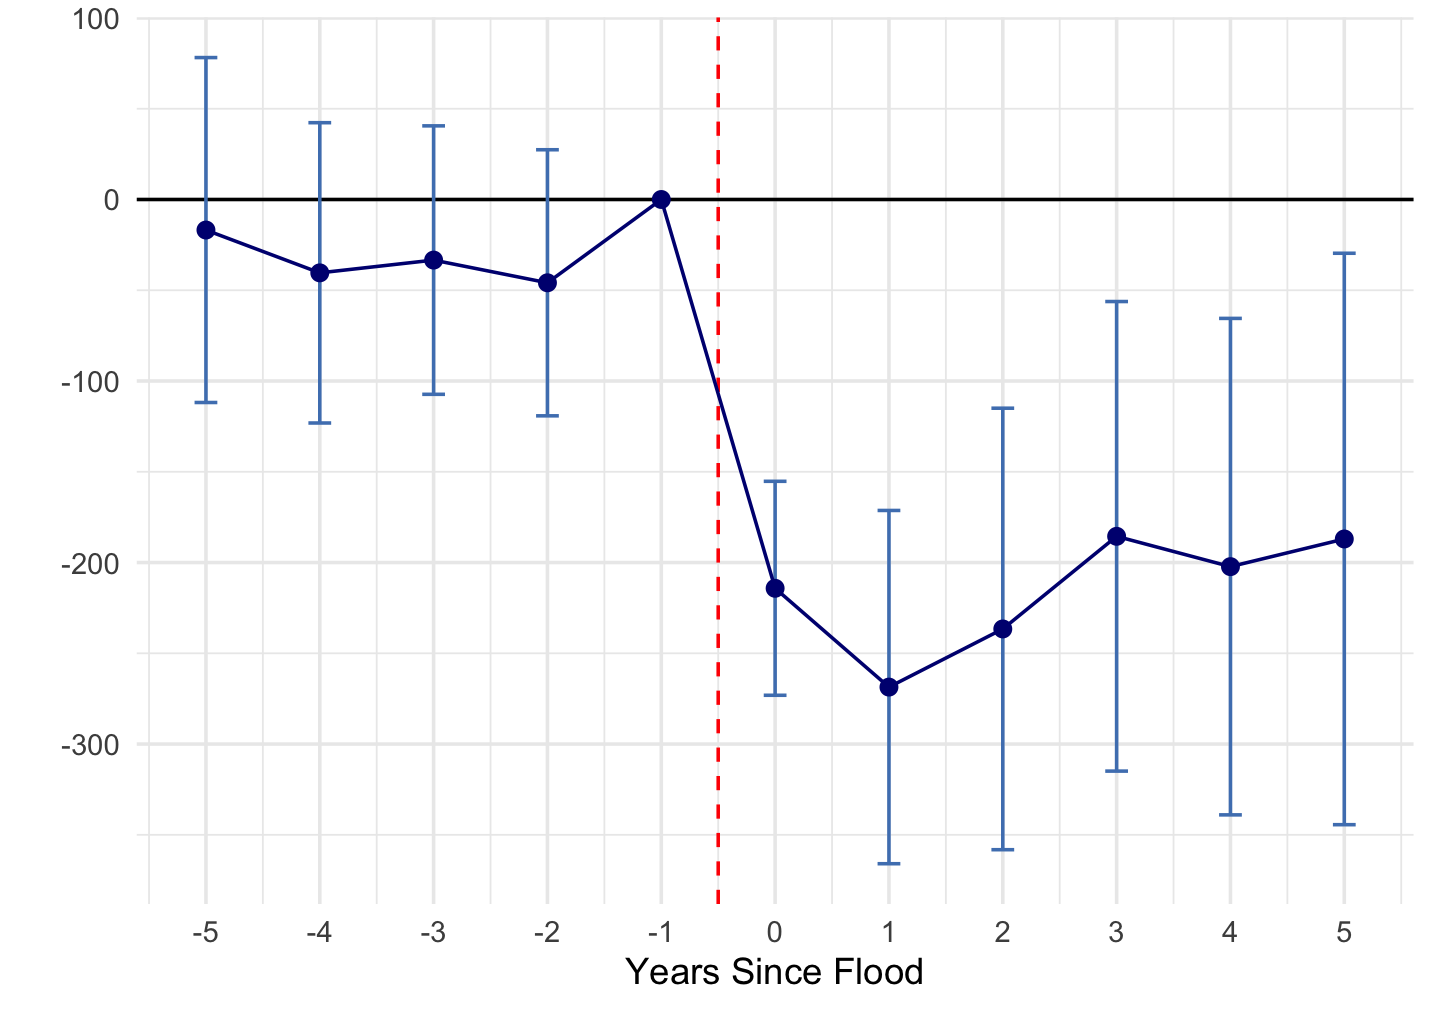
\includegraphics[width=\linewidth]{figures/Results/Analysis_Firms/AVGWAGE_3112_weighted.png}
    \subcaption{\textbf{Average wage at 31.12}}
    \label{fig:wage3112_firm}
  \end{subfigure}
  \hfill
  \begin{subfigure}[t]{0.49\textwidth}
    \centering
    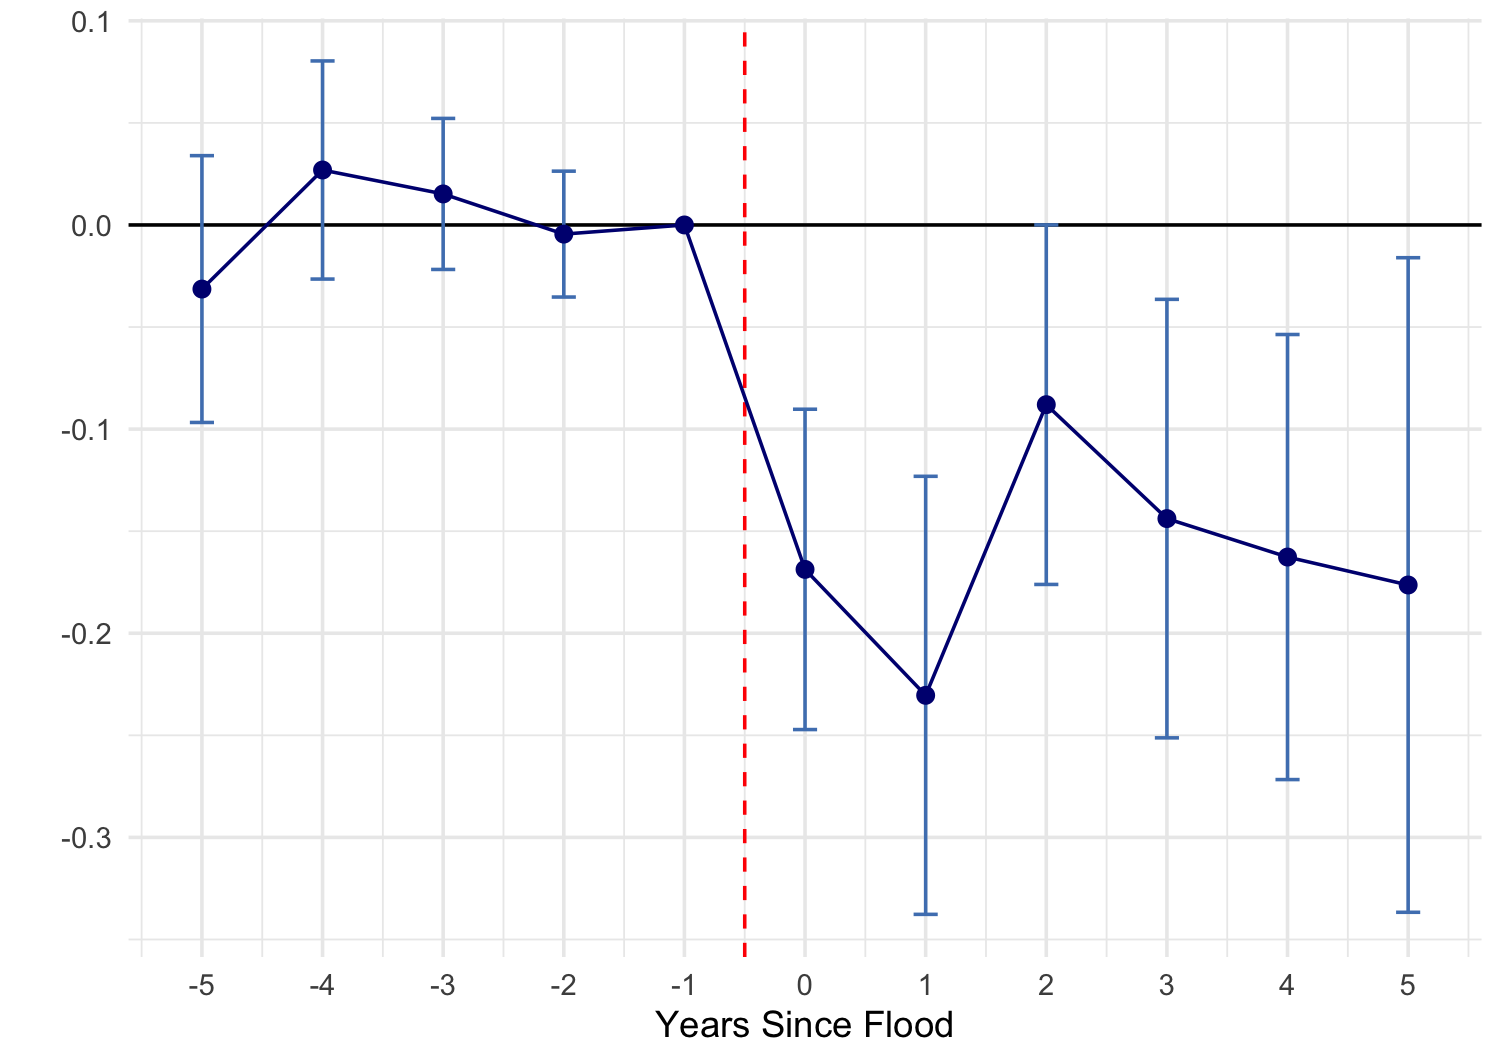
\includegraphics[width=\linewidth]{figures/Results/Analysis_Firms/EFF_3112_weighted.png}
    \subcaption{\textbf{Headcount at 31.12}}
    \label{fig:eff3112_firm}
  \end{subfigure}

  % Second row
  \begin{subfigure}[t]{0.503\textwidth}
    \centering
    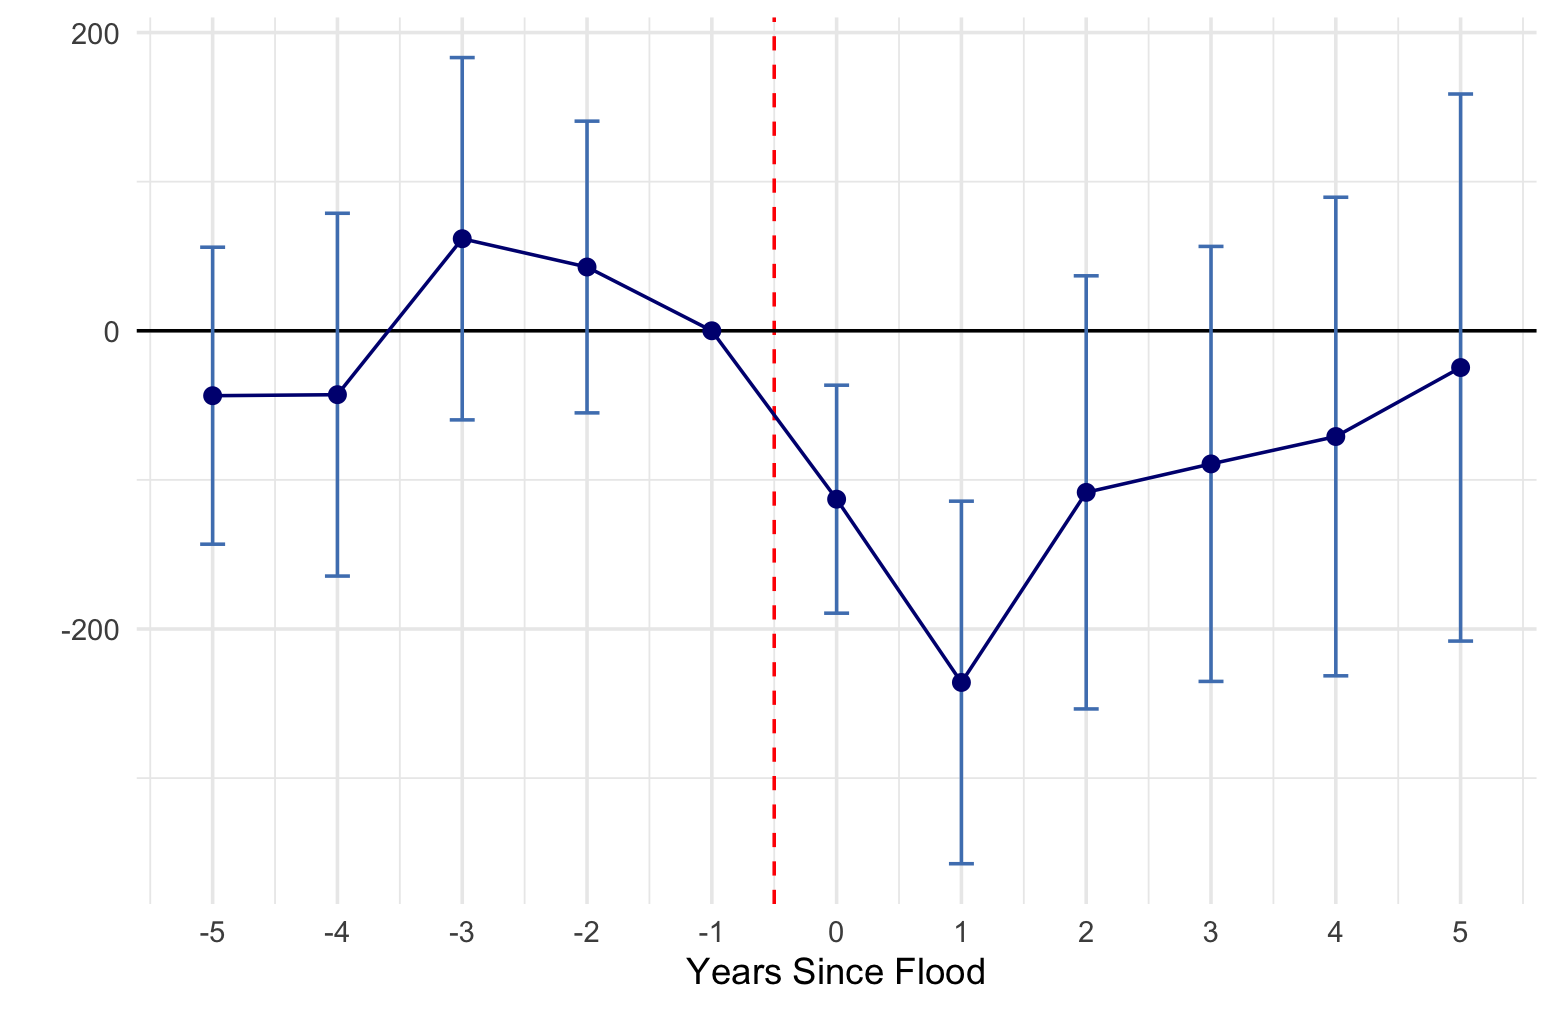
\includegraphics[width=\linewidth]{figures/Results/Analysis_Firms/AVGWAGE yearly.png}
    \subcaption{\textbf{Average Wage Yearly}}
    \label{fig:avg_wage_firm}
  \end{subfigure}
  \hfill
  \begin{subfigure}[t]{0.49\textwidth}
    \centering
    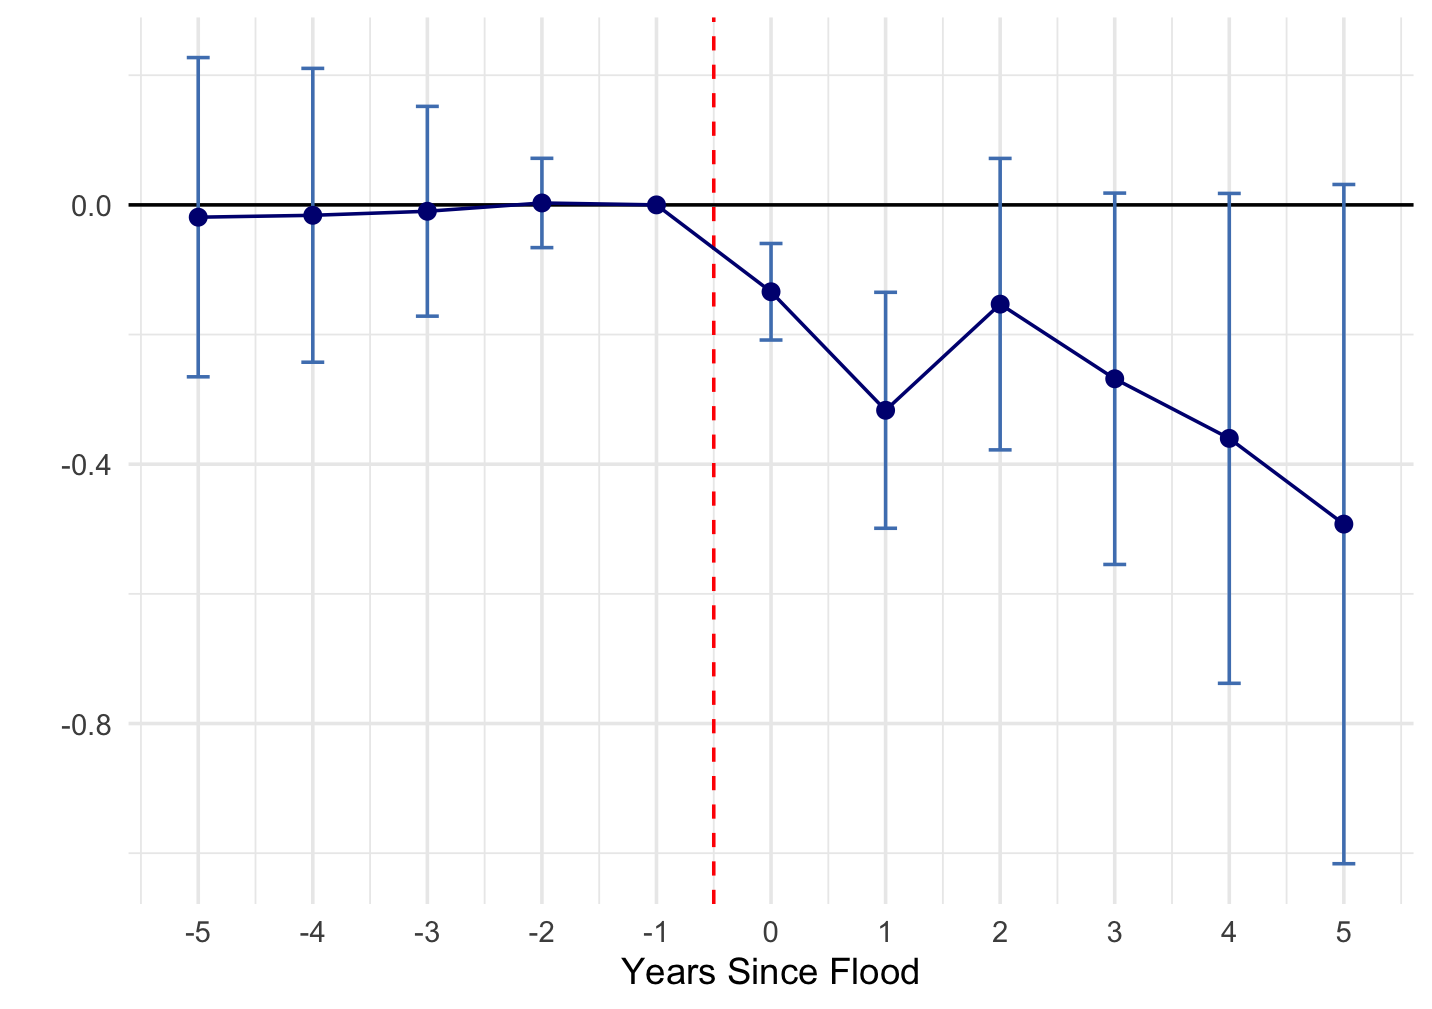
\includegraphics[width=\linewidth]{figures/Results/Analysis_Firms/EFF_ET_MOYEN_weighted.png}
    \subcaption{\textbf{Average Headcount Yearly}}
    \label{fig:avg_eff_firm}
  \end{subfigure}
  
  %\caption*{\textit{Note:} thee fixed effects,,.. the table with pooled estimates is shown in Table..}

  
\end{figure}

%%%%%%%%%%%%%%%%%%%%%%%%%%%%%%%%%%%%%%%%%%%%%%%%%%%%%%%%%
%%%%%%%%%%%%%%%%%%%%%%%%%%%%%%%%%%%%%%%%%%%%%%%%%%%%%%%%%




\begin{table}[!htbp]
\centering
\caption{\textbf{Table \ref{tab:lpdid_pooled}}: \textsc{Main LP-DiD Estimates at Establishment Level}}
\label{tab:lpdid_pooled}

\resizebox{16.3cm}{!}{
\begin{tabular}{@{\extracolsep{6pt}}p{6.5cm}cccccc}
\\[-1.8ex]\hline
\hline \\[-1.8ex]
& \multicolumn{6}{c}{\textit{Dependent variable:}} \\
\cline{2-7}
\\[-1.8ex] 
& Employment 31.12 & Wages 31.12 & Temporary contracts & Employment Yearly & Hourly Wages & Total Revenue \\
&  &  &  & & & \\
\hline \\[-1.8ex]

\textbf{Post-Treatment Average Effect} \\[0.15em]
\textit{A. Full Sample} \\[0.15em]
Treated (=1) $\times$ Post (=1) 
& $-$0.151$^{***}$ & $-$233.62$^{***}$ & $-$0.0026 & $-$0.424 & $-$0.055 & 486.689 \\
& (0.063)           & (77.57)         & (0.0025)     & (0.287) & (0.033) & (263.316) \\[0.75em]

\textit{B. By strata} \\[0.15em]
Mono-establishment (=1) 
& $-$0.022 & $-$524.13$^{***}$ & $-$0.0052 & $-$0.0070 & $-$0.170$^{**}$ & $-$15.388 \\
& (0.012)  & (127.62)          & (0.0047)  & (0.023)   & (0.079)         & (20.013) \\[0.25em]

Litorale (=1) 
& $-$0.134$^{*}$ & $-$114.26 & $-$0.0130$^{**}$ & $-$0.072 & 0.077 & 393.69 \\
& (0.180)        & (191.26)  & (0.0059)         & (0.347)  & (0.076)  & (448.64) \\[0.25em]

Mono-estab. (=1) $\times$ Litorale (=1) 
&   $-$0.031     &  $-$681.695$^{**}$  &  $-$0.038$^{**}$  &  $-$0.021     &   0.119     & $-$29.77 \\
&    (0.043)    &   (288.359)     &      ($-$0.0066)     &   (0.051)     &  (0.144)      & (19.13) \\[0.5em]

\hline \\[-1.8ex]
Total observations         & 6.82M & 6.82M & 6.82M & 6.82M & 6.82M & 6.82M \\
\textit{Fixed effects}     &       &       &       &       &       & \\
Year                       & Yes   & Yes   & Yes   & Yes   & Yes   & Yes \\
Commune                    & Yes   & Yes   & Yes   & Yes   & Yes   & Yes \\
Flood risk group $\times$ Section $\times$ Year 
                          & Yes   & Yes   & Yes   & Yes   & Yes   & Yes \\
Clustered SEs at establishment   
                          & Yes   & Yes   & Yes   & Yes   & Yes   & Yes \\

\hline
\hline \\[-1.8ex]
\multicolumn{7}{p{23cm}}{\textit{Notes:} Each column reports pooled Local Projection DiD coefficients for the post-treatment period (mean of event times $k = 0$ to $5$). Robust standard errors clustered at the establishment level (\texttt{SIRET}) in parentheses. $^{*}p<0.10$; $^{**}p<0.05$; $^{***}p<0.01$.}
\end{tabular}}
\end{table}




\\
\\
\vspace{\baselineskip}

The subsample regression results indicate that the negative impact of flooding on firm wages is more pronounced for firms with a single establishment. This is consistent with the notion that multi-establishment firms can reallocate activity across locations and thereby cushion the effects of local shocks, whereas mono-establishment firms lack this adjustment margin and are thus more vulnerable. Beyond this dimension, it would be interesting to examine the role of tangible asset intensity, since physical capital such as plants, equipment, and warehouses is particularly susceptible to flood damage.

%Firms located in cities with low government quality, indicating that poor public choices and inefficient/incompetent city management can exacerbate the negative impact of flooding? Other interesting strata would be: urban, 

%Check for france, e.g., the Amount of municipal "green" investments to fedine "green communes, Then variables such as litorale, urban, income category, disburment of “fonds Barnier” in France;  as well as the Fond Vert. firm size can be used! FIrms with more intangible assets! only manufacturing so "active etablussment", like \cite{erda2024disasters}. Our subsample regression results reveal that the negative impact of flooding on firm wages and labour demand is more pronounced for firms with single stablishemnts. OR i could check with more intensive tangible asset investment, likely because tangible capital assets such as plants, equipment and warehouses can suffer significant damages due to flooding. \\we find that the negative impact of flooding on firm performance is significantly greater for firms facing tight financial constraints.\\ \href{https://pmc.ncbi.nlm.nih.gov/articles/PMC9278787/#pone.0271309.ref001}{source}


Finally, there is potential attrition at the extensive margin: plants that exit remain recorded in the DADS with zero workers, but may disappear entirely from the revenue panel. This can generate survivorship bias that dampens the estimated effects on sales or profits unless exits are explicitly coded as zero. Survival analyses, which are not undertaken in this paper, can be found in \cite{erda2024disasters}, \cite{fatica2024floods}, and \cite{clo2024impact}. A further limitation concerns the treatment definition. Commune-level flood dummies may adequately capture labor market disruptions, but they are likely to attenuate estimated effects on output when only part of an industrial zone is affected. Future specifications could address this by interacting the treatment with flood depth or with the share of commune area inundated, thereby capturing variation in exposure intensity more accurately.


\section{Sectoral heterogeneity in the impact of flooding}

To understand how the effects of flooding vary across the economy, I explore heterogeneity along a key dimension: the sector of activity. Figure~\ref{fig:firms_results_heter} displays event study estimates of average wage and headcount at the end of year ($31.12$), disaggregated by sector. Several patterns emerge.

\begin{figure}[htbp]
\centering
\caption{\textbf{Figure \ref{fig:firms_results_heter}:} Sectoral heterogeneity in the impact of flooding}
\label{fig:firms_results_heter}
\begin{subfigure}[t]{0.49\textwidth}
\centering
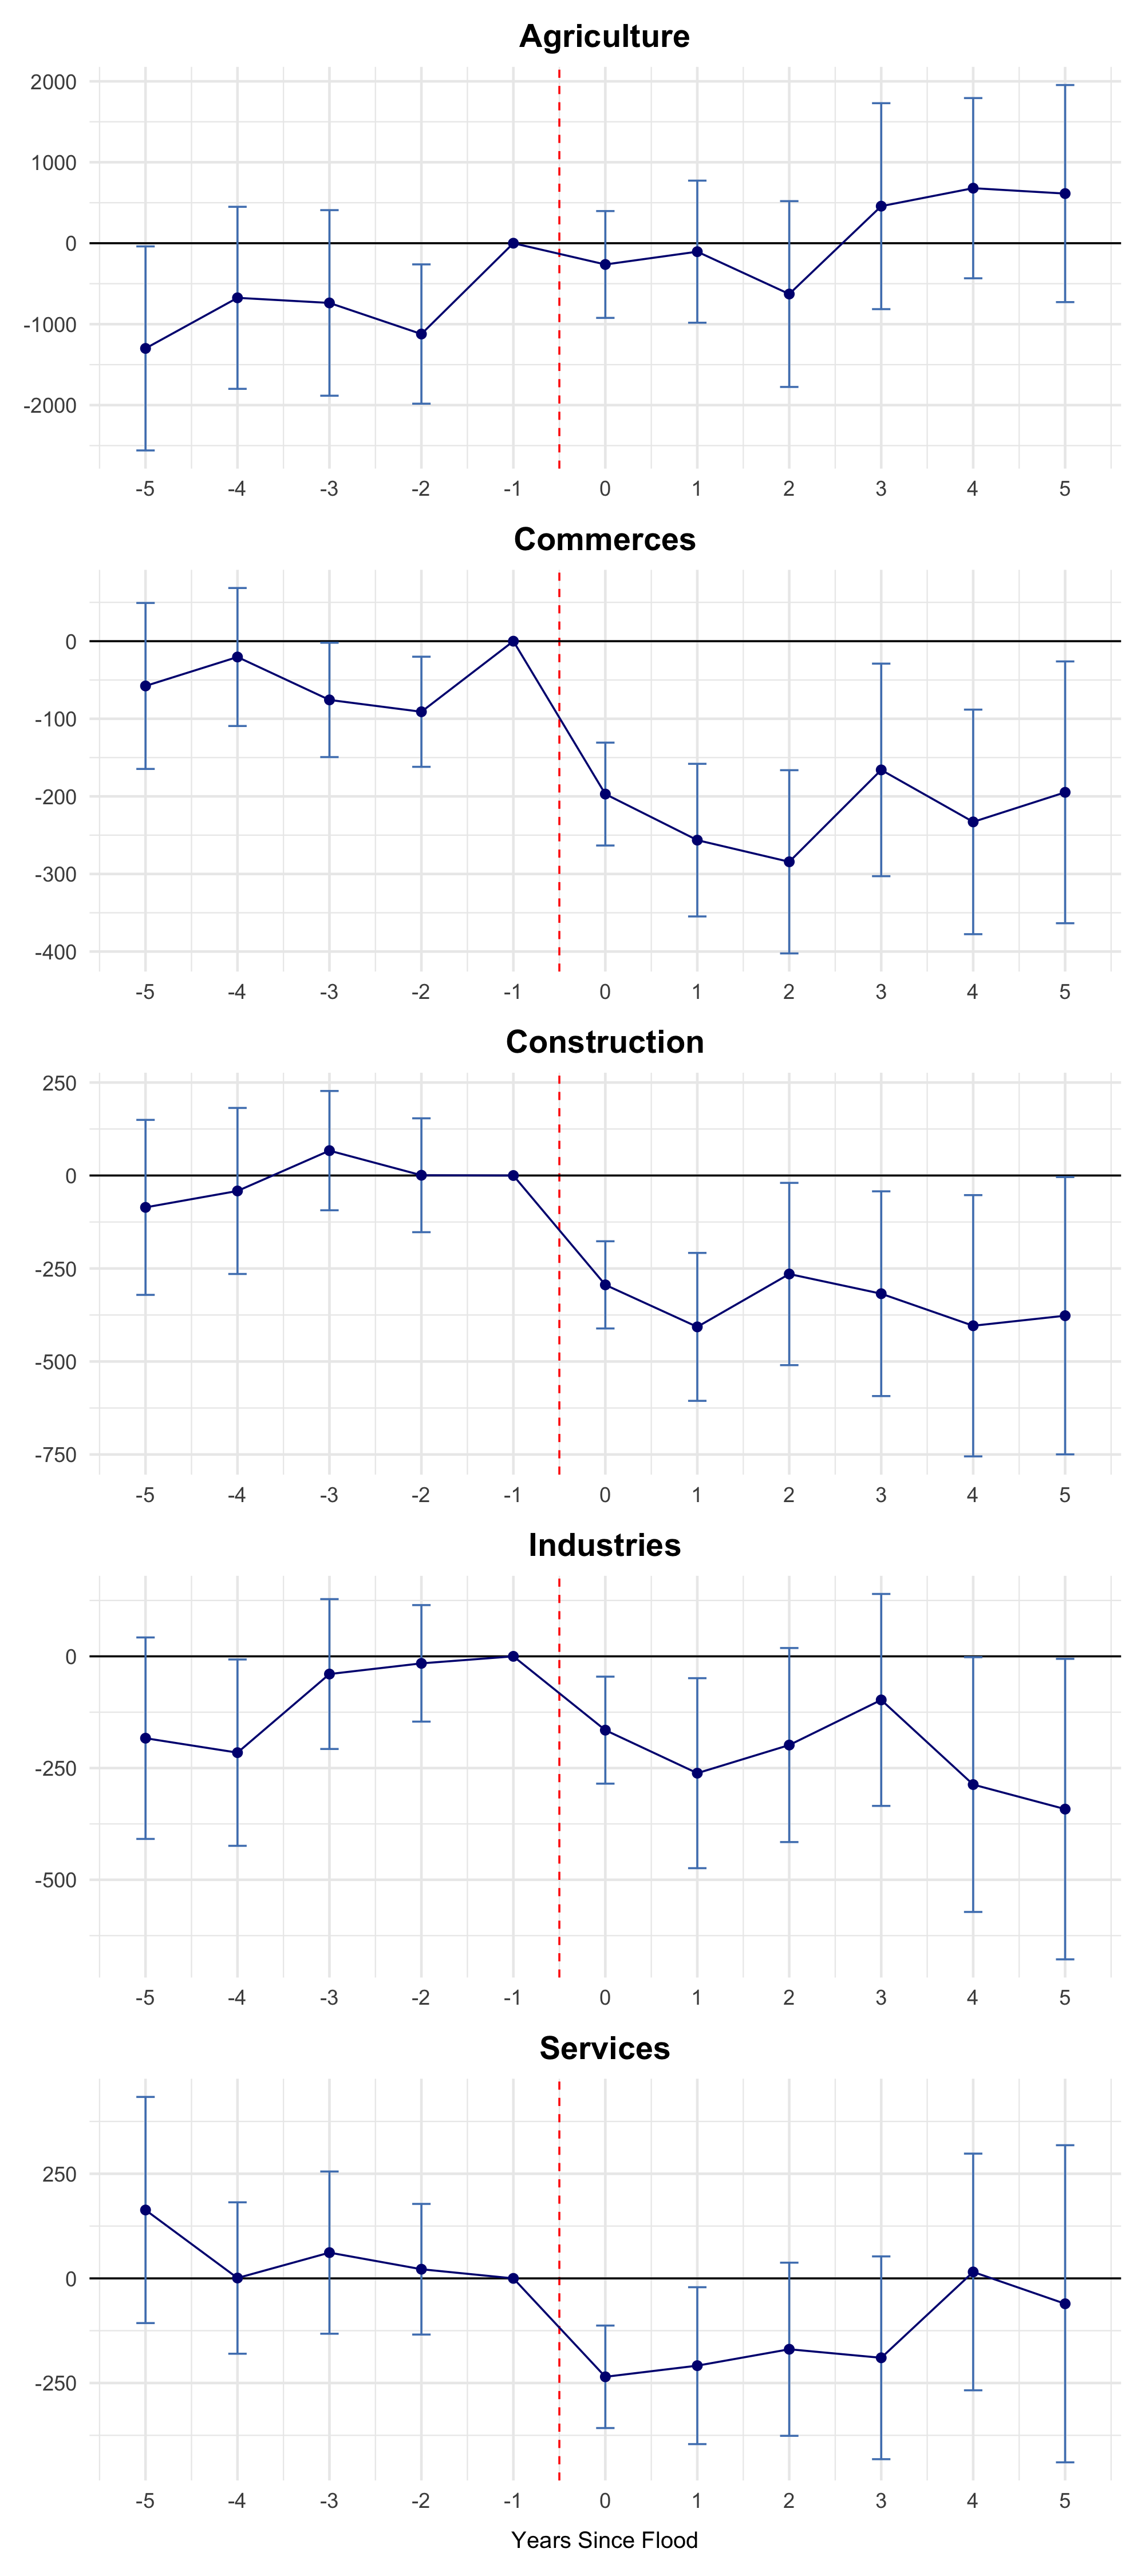
\includegraphics[width=\linewidth]{figures/Results/Analysis_Firms/AVGWAGE_3112_Sectors.png}
\subcaption{\textbf{Average wage at 31.12}}
\label{fig:avg_wage_firm_heter}
\end{subfigure}
\hspace{0.02cm}
\begin{subfigure}[t]{0.49\textwidth}
\centering
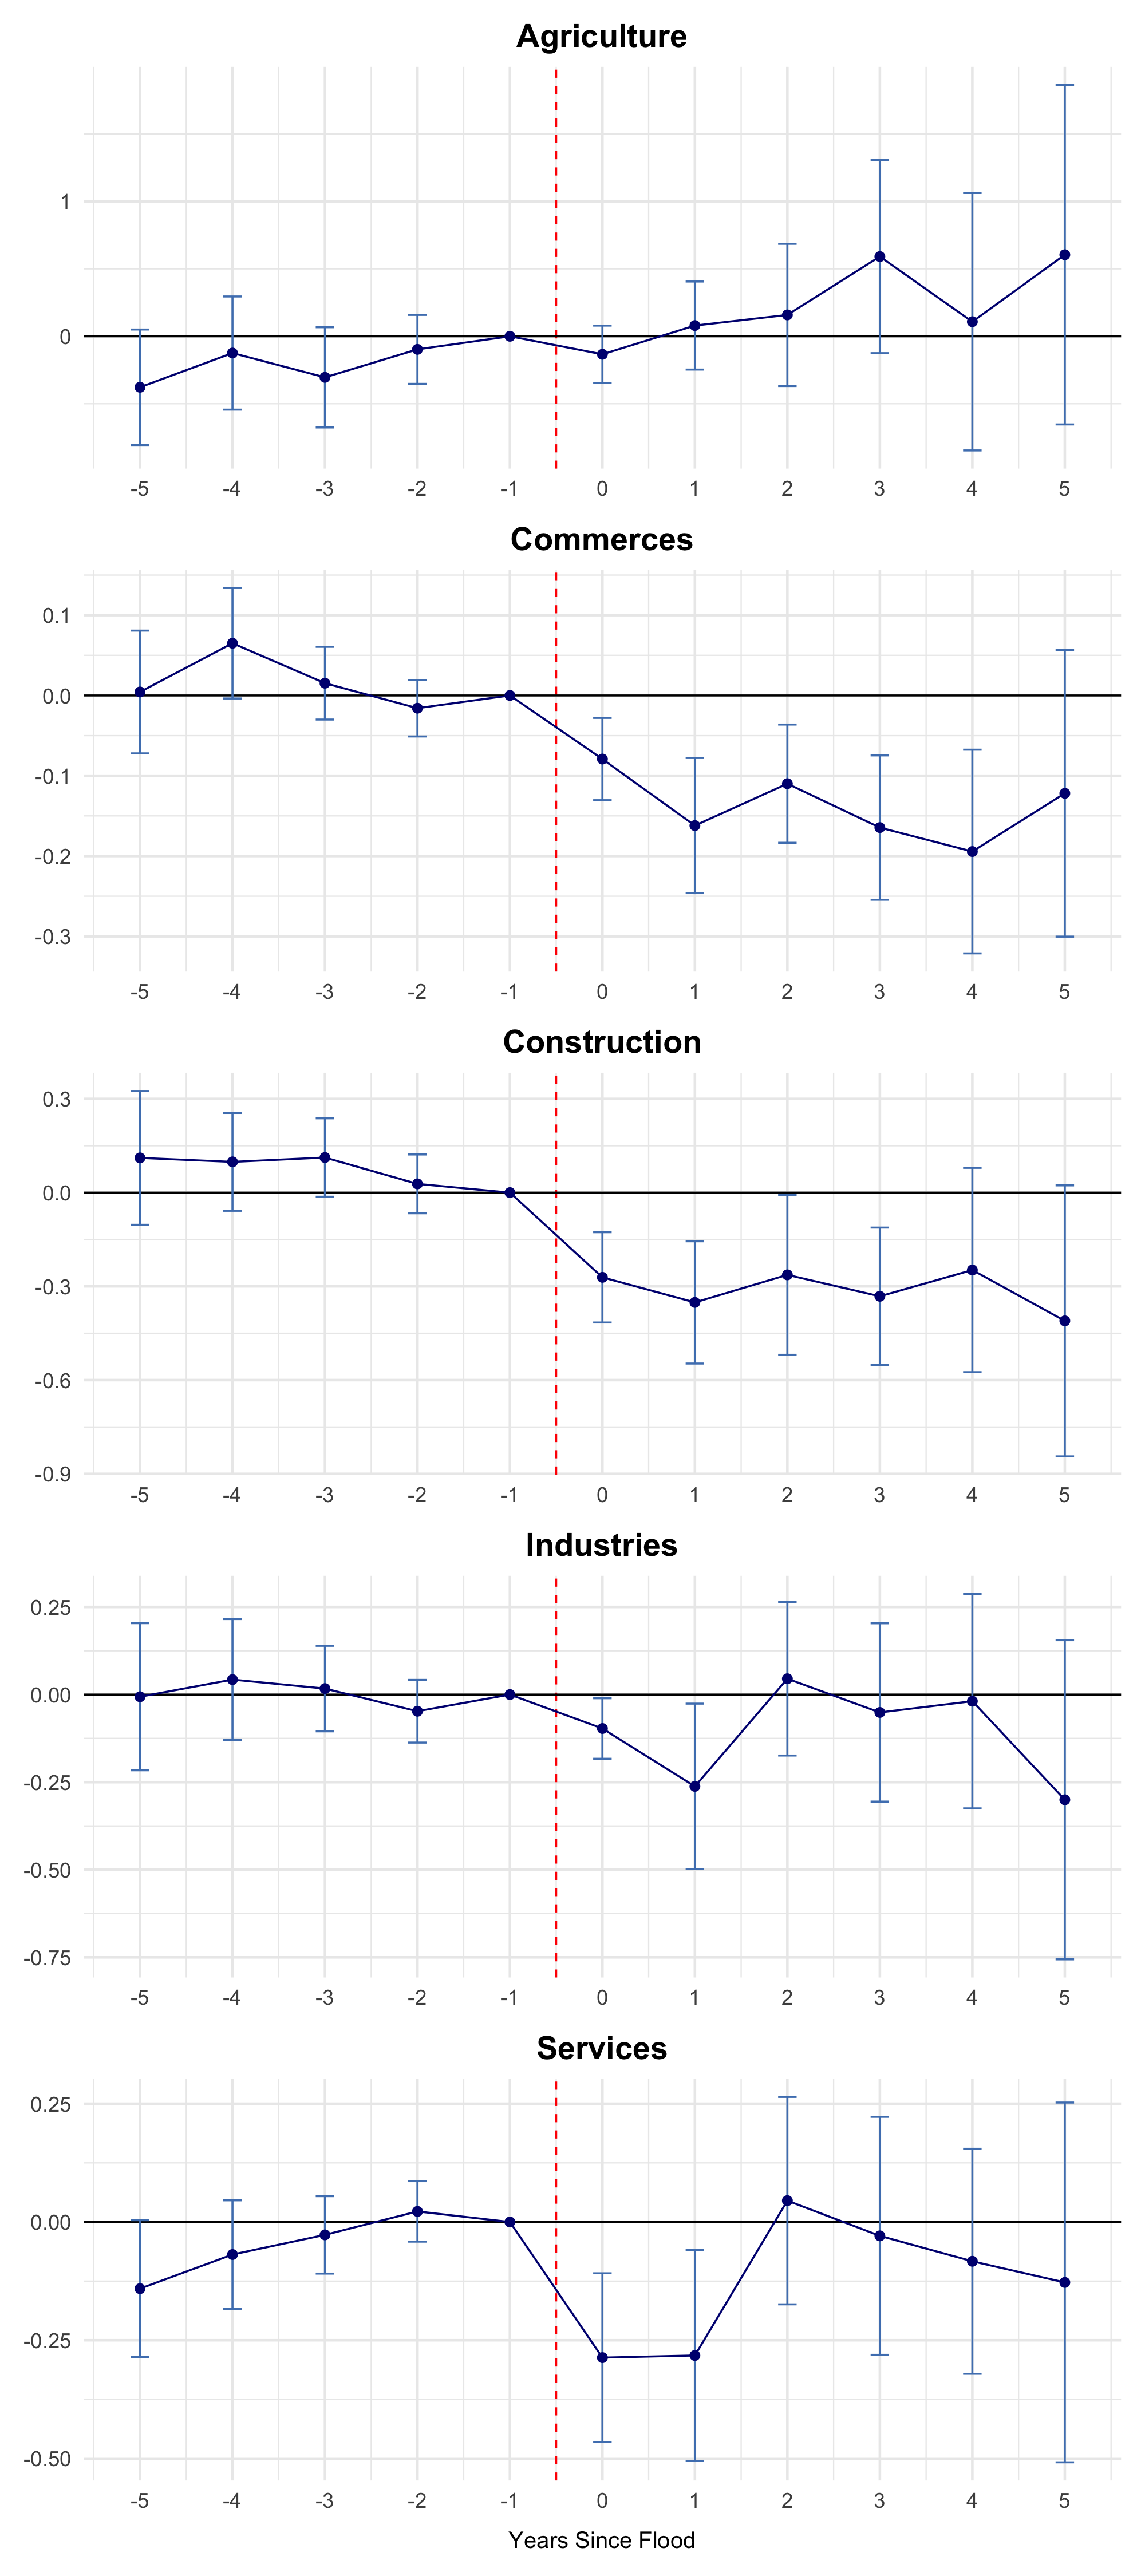
\includegraphics[width=\linewidth]{figures/Results/Analysis_Firms/EFF_3112_Sectors.png}
\subcaption{\textbf{Headcount at 31.12}}
\label{fig:eff3112_firm_heter}
\end{subfigure}

\vspace{0.8em}
\end{figure}


First, the parallel-trends assumption appears to hold across all sector panels: coefficients on the leads ($k = -5$ to $k = -2$) are statistically indistinguishable from zero, supporting the identifying assumption of the LP-DiD design. Turning to the post-flood dynamics, Panels (a) and (b) show that all sectors except agriculture experience some decline in average wages and employment, though the intensity and persistence vary considerably.

In commerce, employment drops sharply—by about 20\% in the first year after a flood ($k=1$)—and losses persist through $k=5$. Construction suffers the most severe and prolonged effects, with employment falling by up to 30\% around $k=3$, despite the potential for increased reconstruction demand. These results indicate that both sectors are especially vulnerable to flooding, likely due to their reliance on physical storefronts, infrastructure, and on-site activity. Services also show a persistent decline, though of a more moderate scale (10–15\%). This suggests that local service providers face sustained challenges after floods, stemming from demand shifts, commuting disruptions, or damage to premises, and they may be unable to reorganize production flexibly, as argued by \cite{indaco2021hurricanes}.

By contrast, the industrial sector shows little to no systematic response: coefficients fluctuate around zero and remain statistically insignificant, pointing to greater flood resilience, possibly due to larger capital buffers, insurance coverage, or geographic insulation from flood-prone areas. Similarly, the agricultural sector exhibits high variance but no consistent directional effect, with noisy estimates centered around zero. This pattern may reflect strong adaptation mechanisms in farming or substantial heterogeneity within the sector.

Taken together, these results suggest that sectors relying heavily on localized retail activity, manual labor, and in-person service delivery (commerce, construction, many services) bear the brunt of flood impacts. In contrast, sectors with more fixed capital, non-localized markets, or better insurance coverage (industry, agriculture) tend to show quicker recovery or minimal disruption. Importantly, these estimates are based on unweighted regressions. If sectoral heterogeneity shrinks or disappears when using inverse probability weights, this would imply that part of the observed variation reflects selection or compositional differences rather than true underlying disparities in vulnerability. Looking ahead, it would be interesting to examine whether floods also trigger climate transition-type reallocations across industries. Input–output data and information on downstream supplier relationships could help uncover whether flood shocks accelerate structural shifts in production networks.

%%%%%%%%%%%%%%%%%%%%%%%%%%%%%%%%%%%%%%%%%%%%%%%%%%%%%%%%%%%
\section{Commune level analysis}
As aggregate dynamics can differ from individual dynamics, I also run a commune-level analysis, which is the level at which treatment is administratively assigned. It could be interesting in future work to extend this to Local Labour Market (LLM) zones, by interacting commuting zones and APE codes and weighting establishment outcomes by their labor shares in the LLM.
At the commune level, however, the results show no strong or persistent impacts of floods on wages, employment, revenues, share capital, or profits (Figure \ref{fig:IRF_Communes}). This contrasts with the establishment-level results, where floods generated sharp short-term shocks on wages and employment. The absence of aggregate effects highlights recovery dynamics at the municipal scale, consistent with findings in the literature. For instance, \cite{leiter2009creative} document that while Austrian firms suffered severe direct damages from floods, municipal-level aggregates showed relatively rapid recovery due to insurance payouts and redistribution. Similarly, \cite{usman2024going} stress that commune-level indicators often conceal heterogeneity in the impact of extreme weather events, as losses in some establishments are compensated by resilience and adaptation elsewhere in the local economy.
% As aggregate dynamics can differ from individual dynamics, I run a commune level anaylsis, which is the level at which treatmetn is administret. It could be interesting to add to the analysis by running a Local Labour Market level analysis, by creating such zones multiplying Commuting zone and APE codes, and weighting SIRETs outcomes by their labour share in the LLM.

% I see that at commune level there is no such big impacts, this hilights aggreagte recovery dynamics as is pointed out in Leiter or at page. 6 and 28 of going NUTS! SInce no apparetn aggregate impact, they run on communes based on income of commune! I will do this!

% \textbf{Mechanisms:} This designation of flooding episode is place-based, referring to the specific municipalities affected, and primarily triggers compulsory insurance coverage for the damages sustained—it does not automatically unlock substantial public funding for infrastructure reconstruction or direct grants to households and businesses. Nevertheless, it ensures regulated insurance payouts, offering financial relief to those impacted by the floods. \cite{indaco2021hurricanes} finds similar results.


%%%%% Figure: Flood Impacts commune level
\begin{figure}[htp]
  \centering

      \caption{\textbf{Figure \ref{fig:IRF_Communes}:} Flood impacts at the commune level}
    \label{fig:IRF_Communes}
    
  % First row
  \begin{subfigure}[b]{0.33\textwidth}
    \centering
    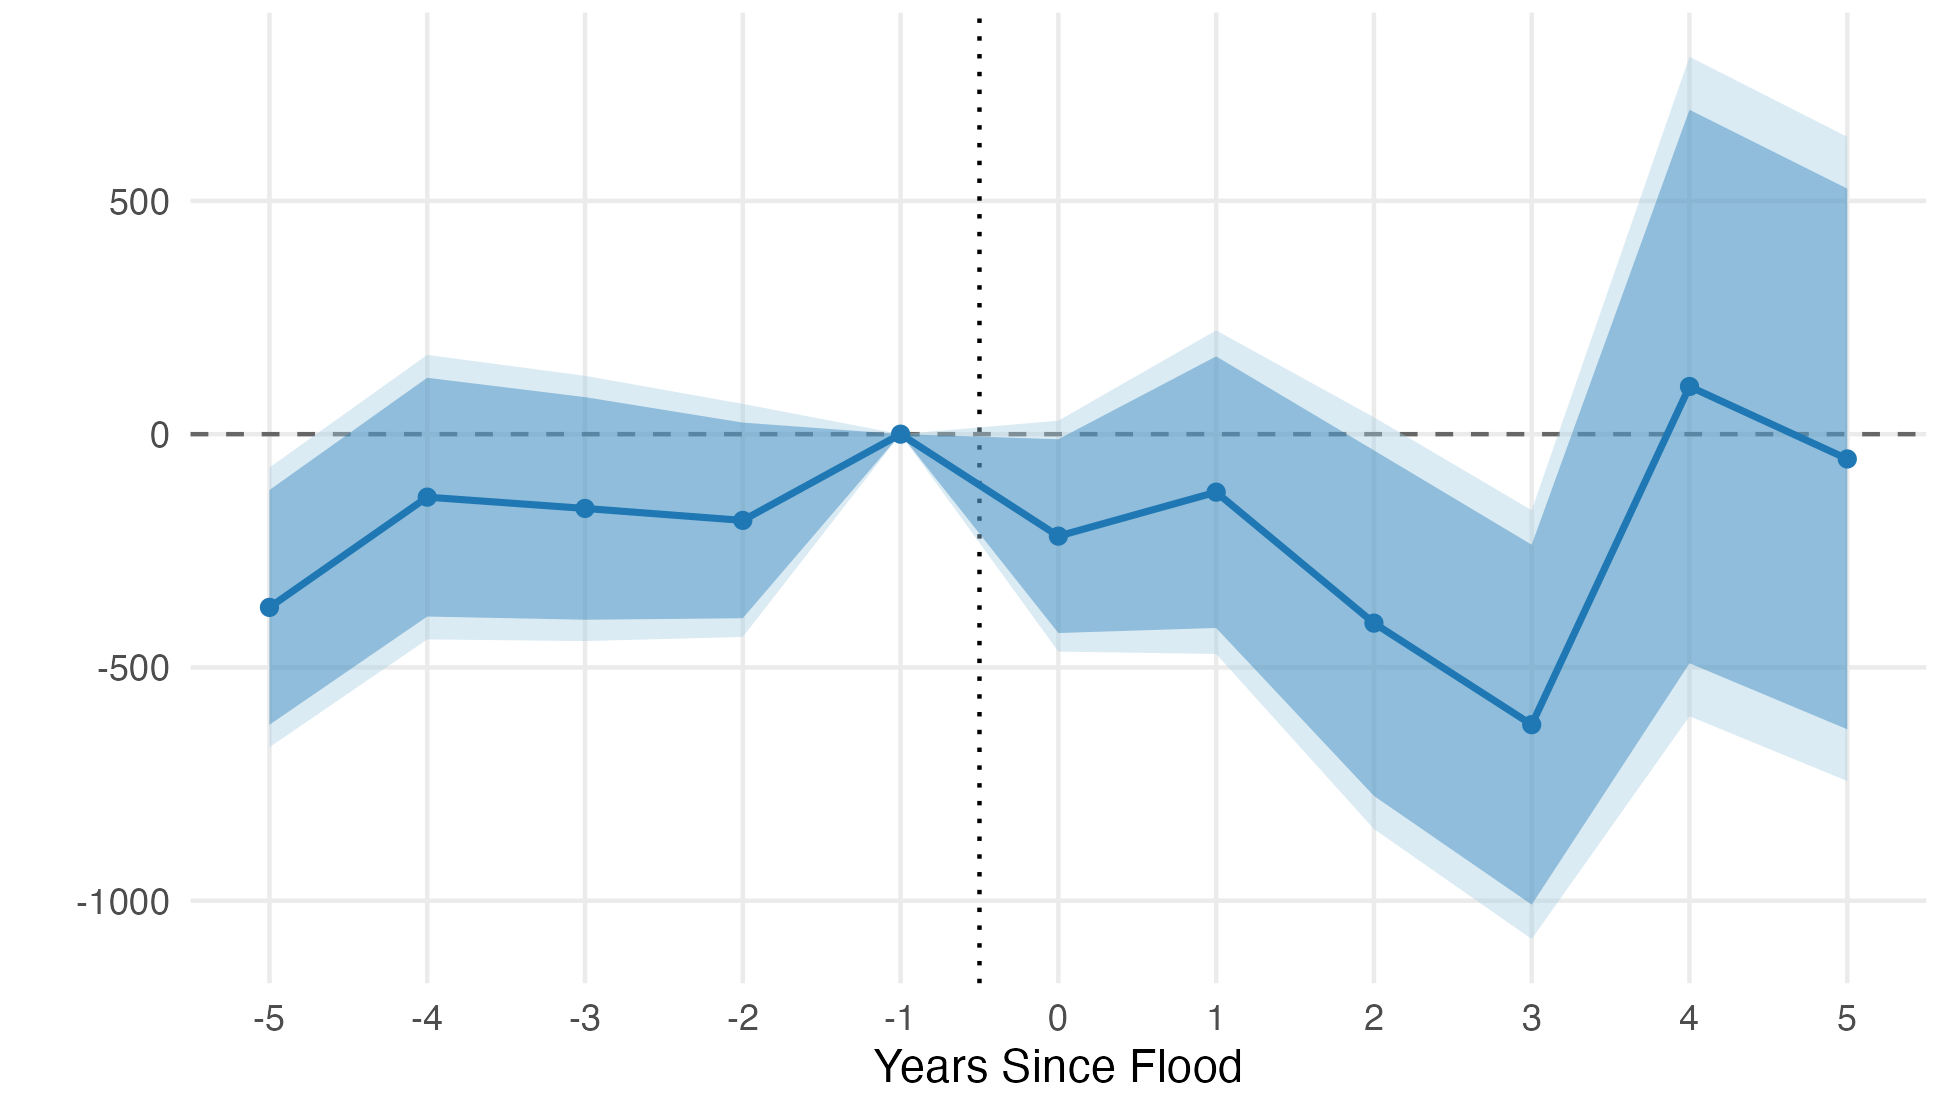
\includegraphics[width=\linewidth]{figures/Results/Analysis_Communes/IRF_AVGWAGE_3112_pooled.png}
    \subcaption{Wages at 31.12}
    \label{}
  \end{subfigure}%
  \begin{subfigure}[b]{0.33\textwidth}
    \centering
    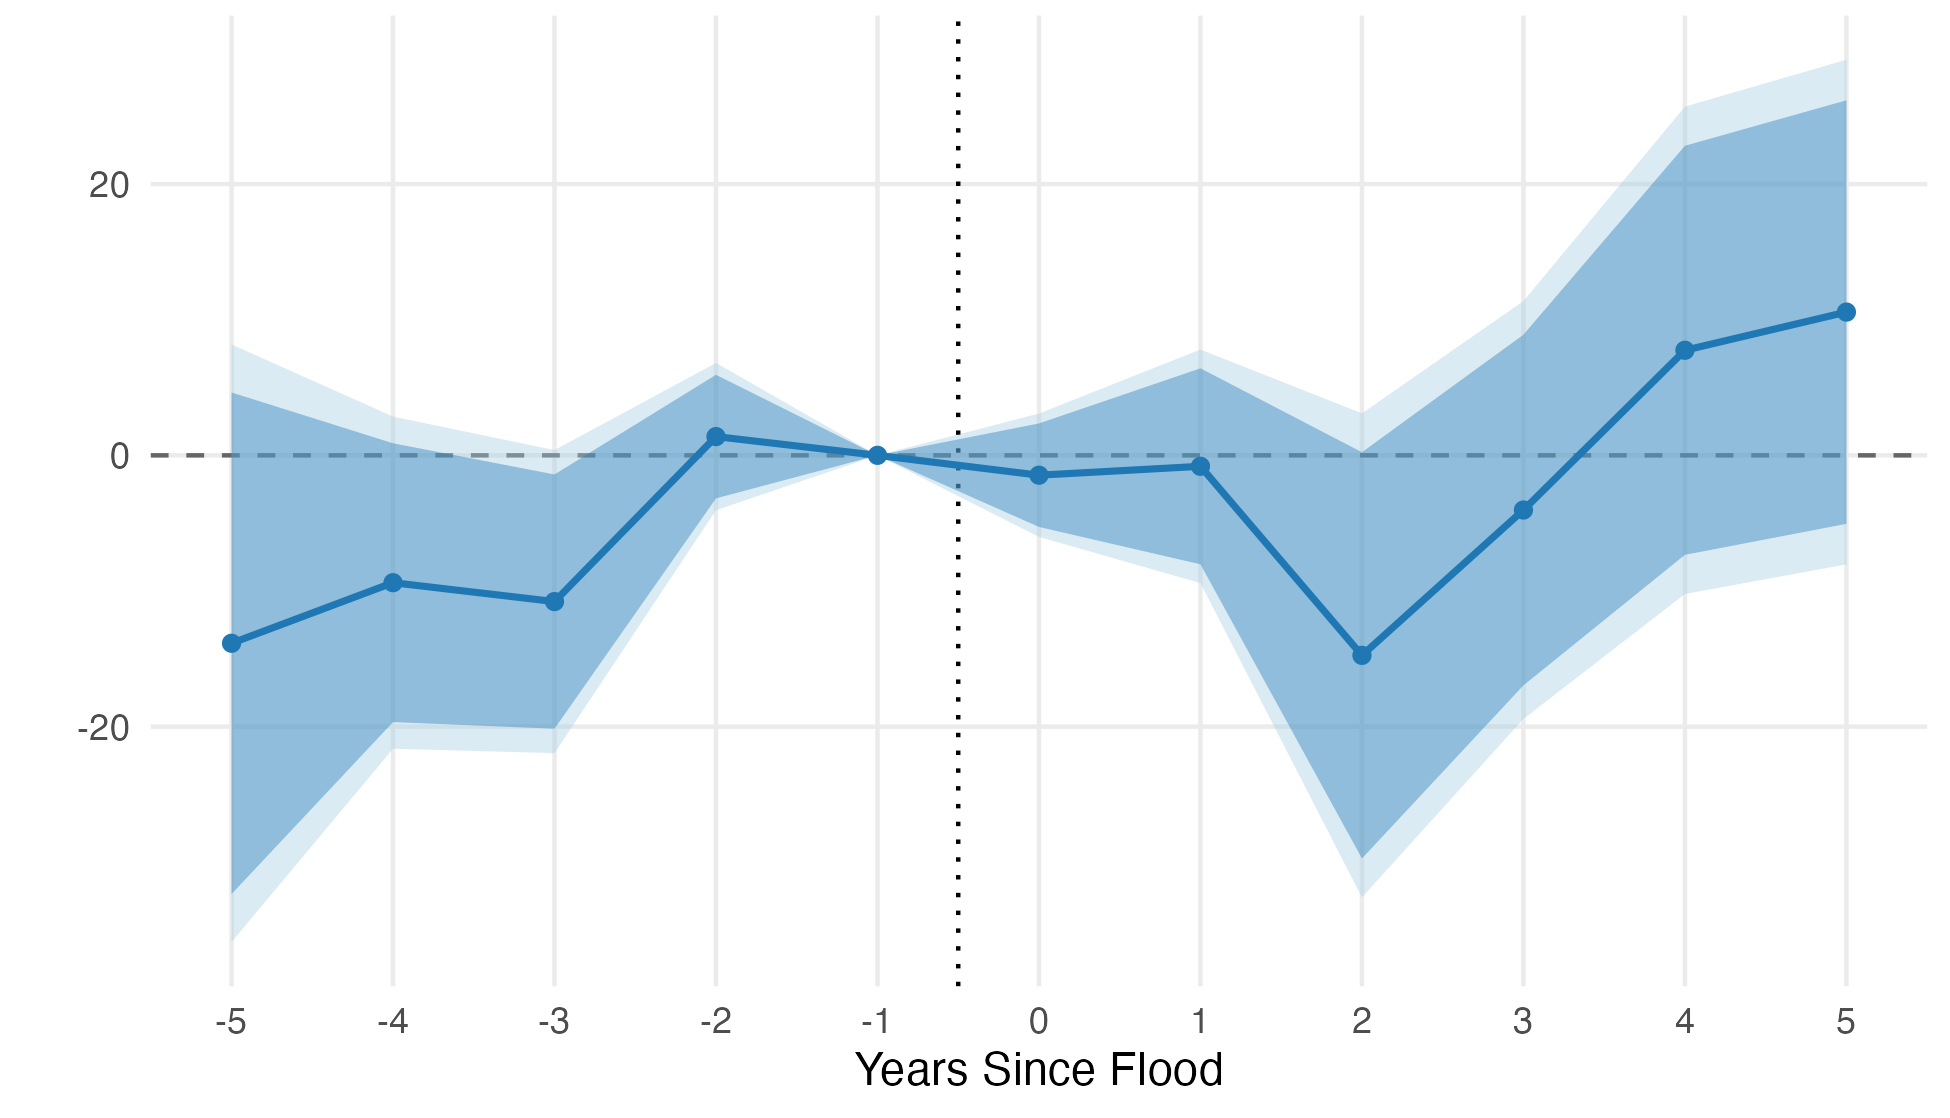
\includegraphics[width=\linewidth]{figures/Results/Analysis_Communes/IRF_EFF_3112_pooled.png}
    \subcaption{Headcount at 31.12}
    \label{fig:eff_all_commmune}
  \end{subfigure}
  \begin{subfigure}[b]{0.33\textwidth}
    \centering
    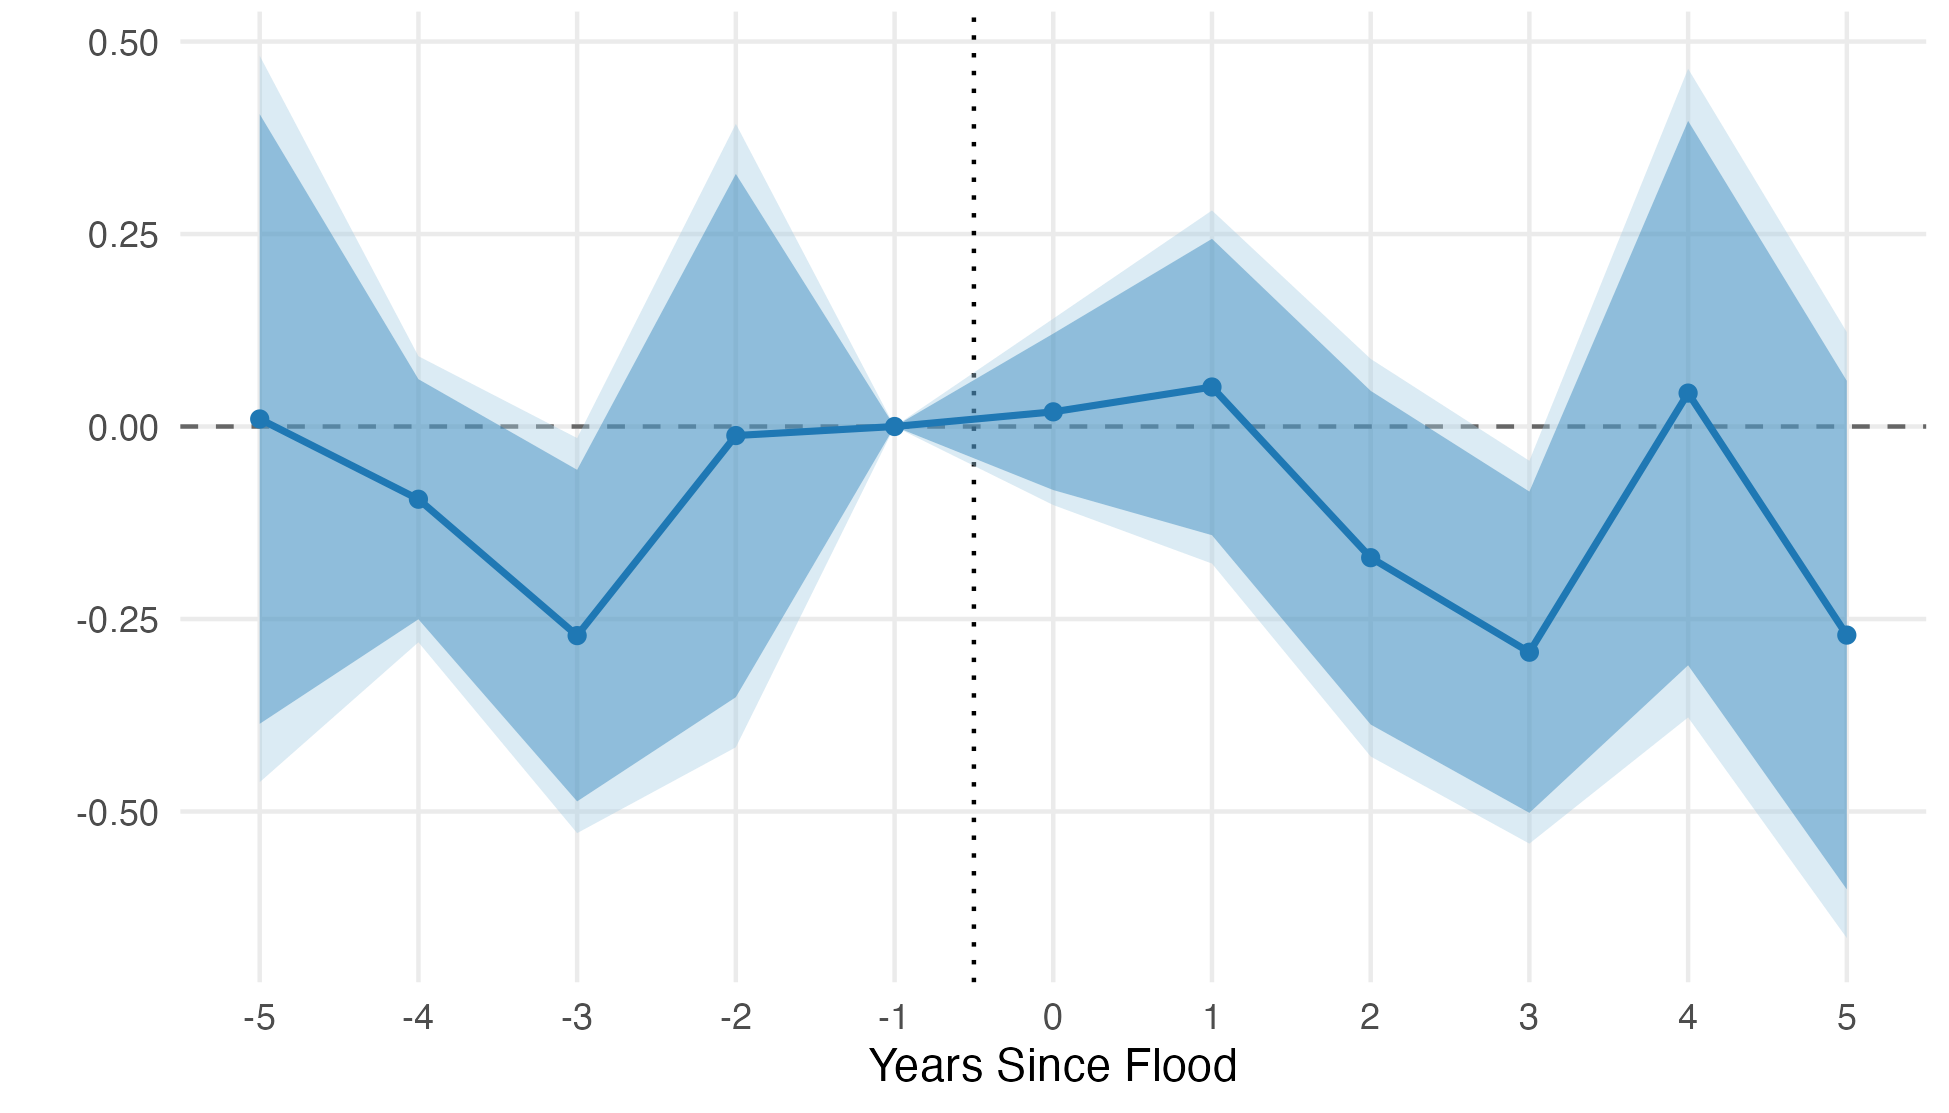
\includegraphics[width=\linewidth]{figures/Results/Analysis_Communes/IRF_HWAGE_3112_pooled.png}
    \subcaption{Hourly Wage}
    \label{}
  \end{subfigure}

 
 \vspace{0.8em}
 
    \begin{subfigure}[b]{0.33\textwidth}
    \centering
    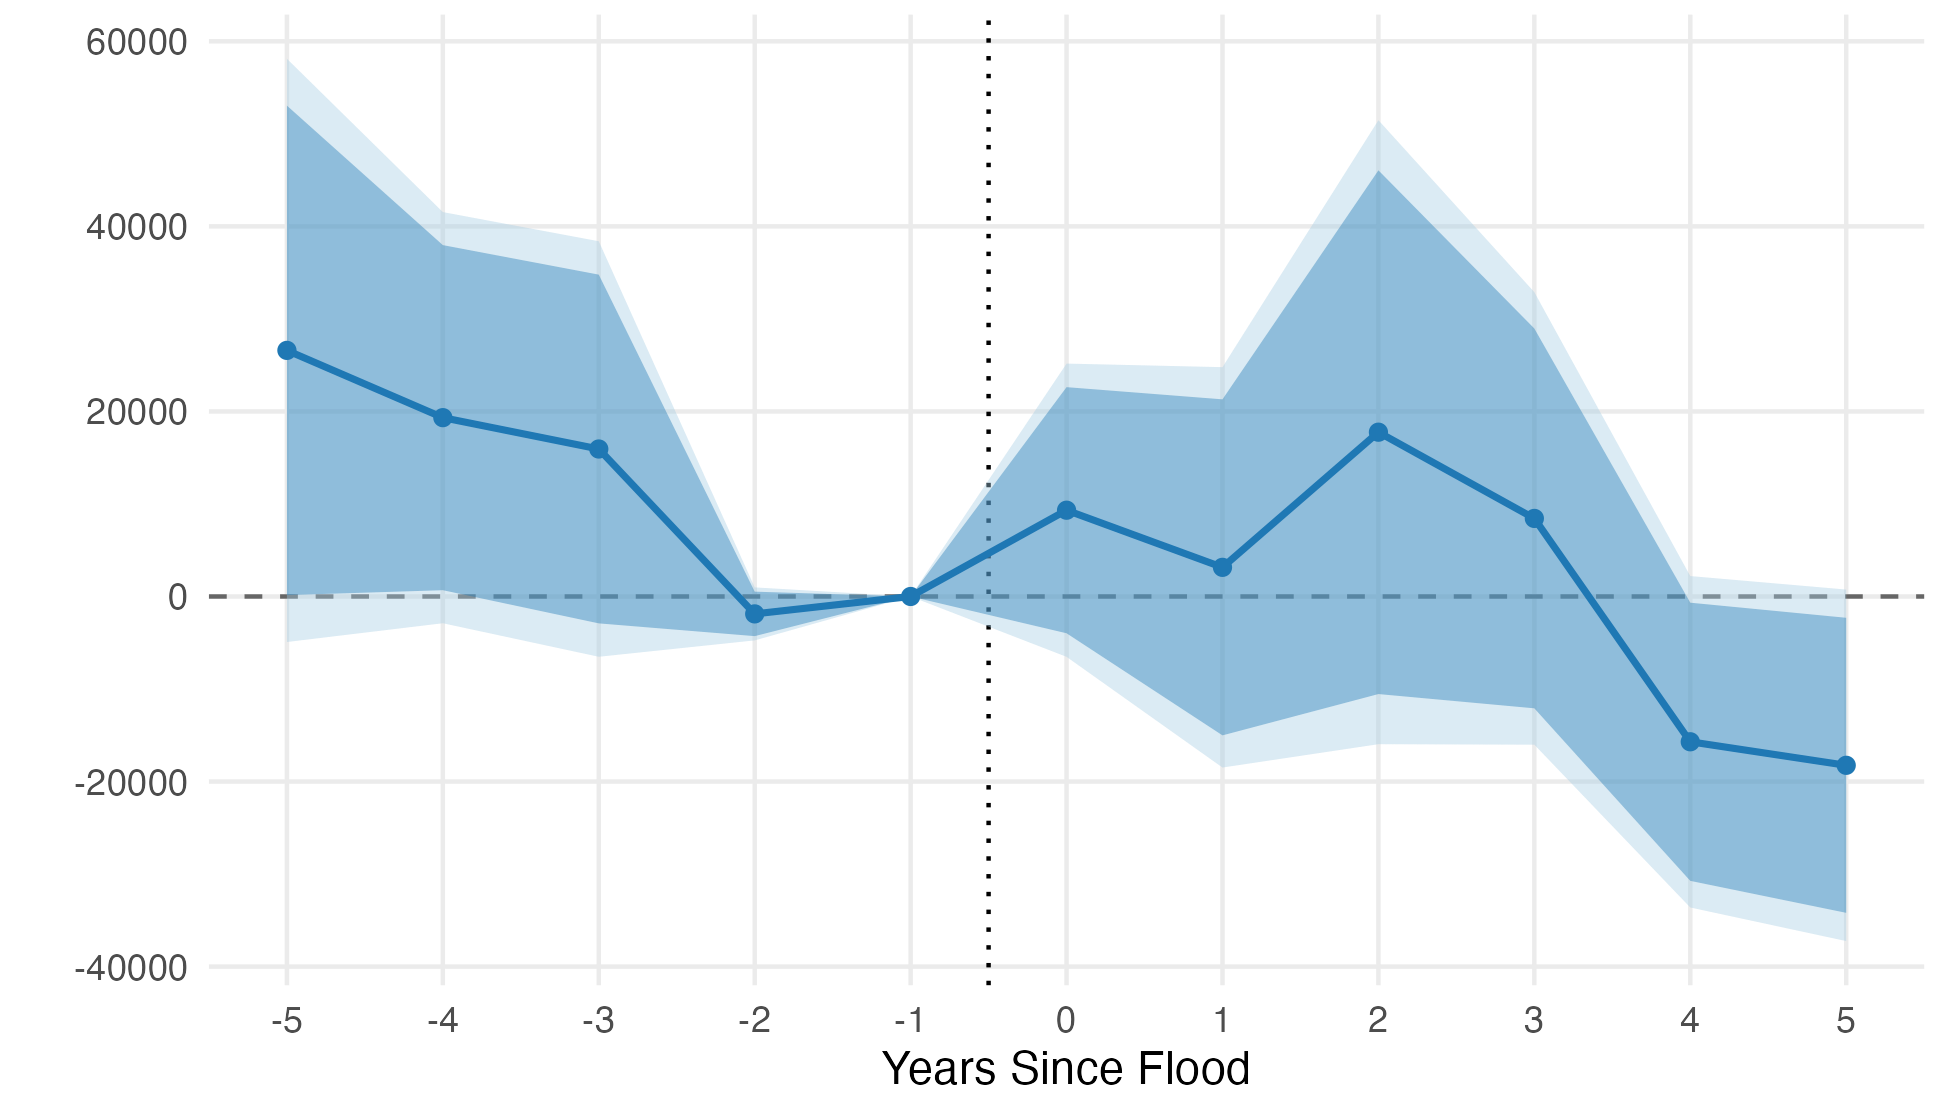
\includegraphics[width=\linewidth]{figures/Results/Analysis_Communes/IRF_redi_r310_SIRET_pooled.png}
    \subcaption{Total Revenue}
    \label{}
  \end{subfigure}
  \begin{subfigure}[b]{0.33\textwidth}
    \centering
    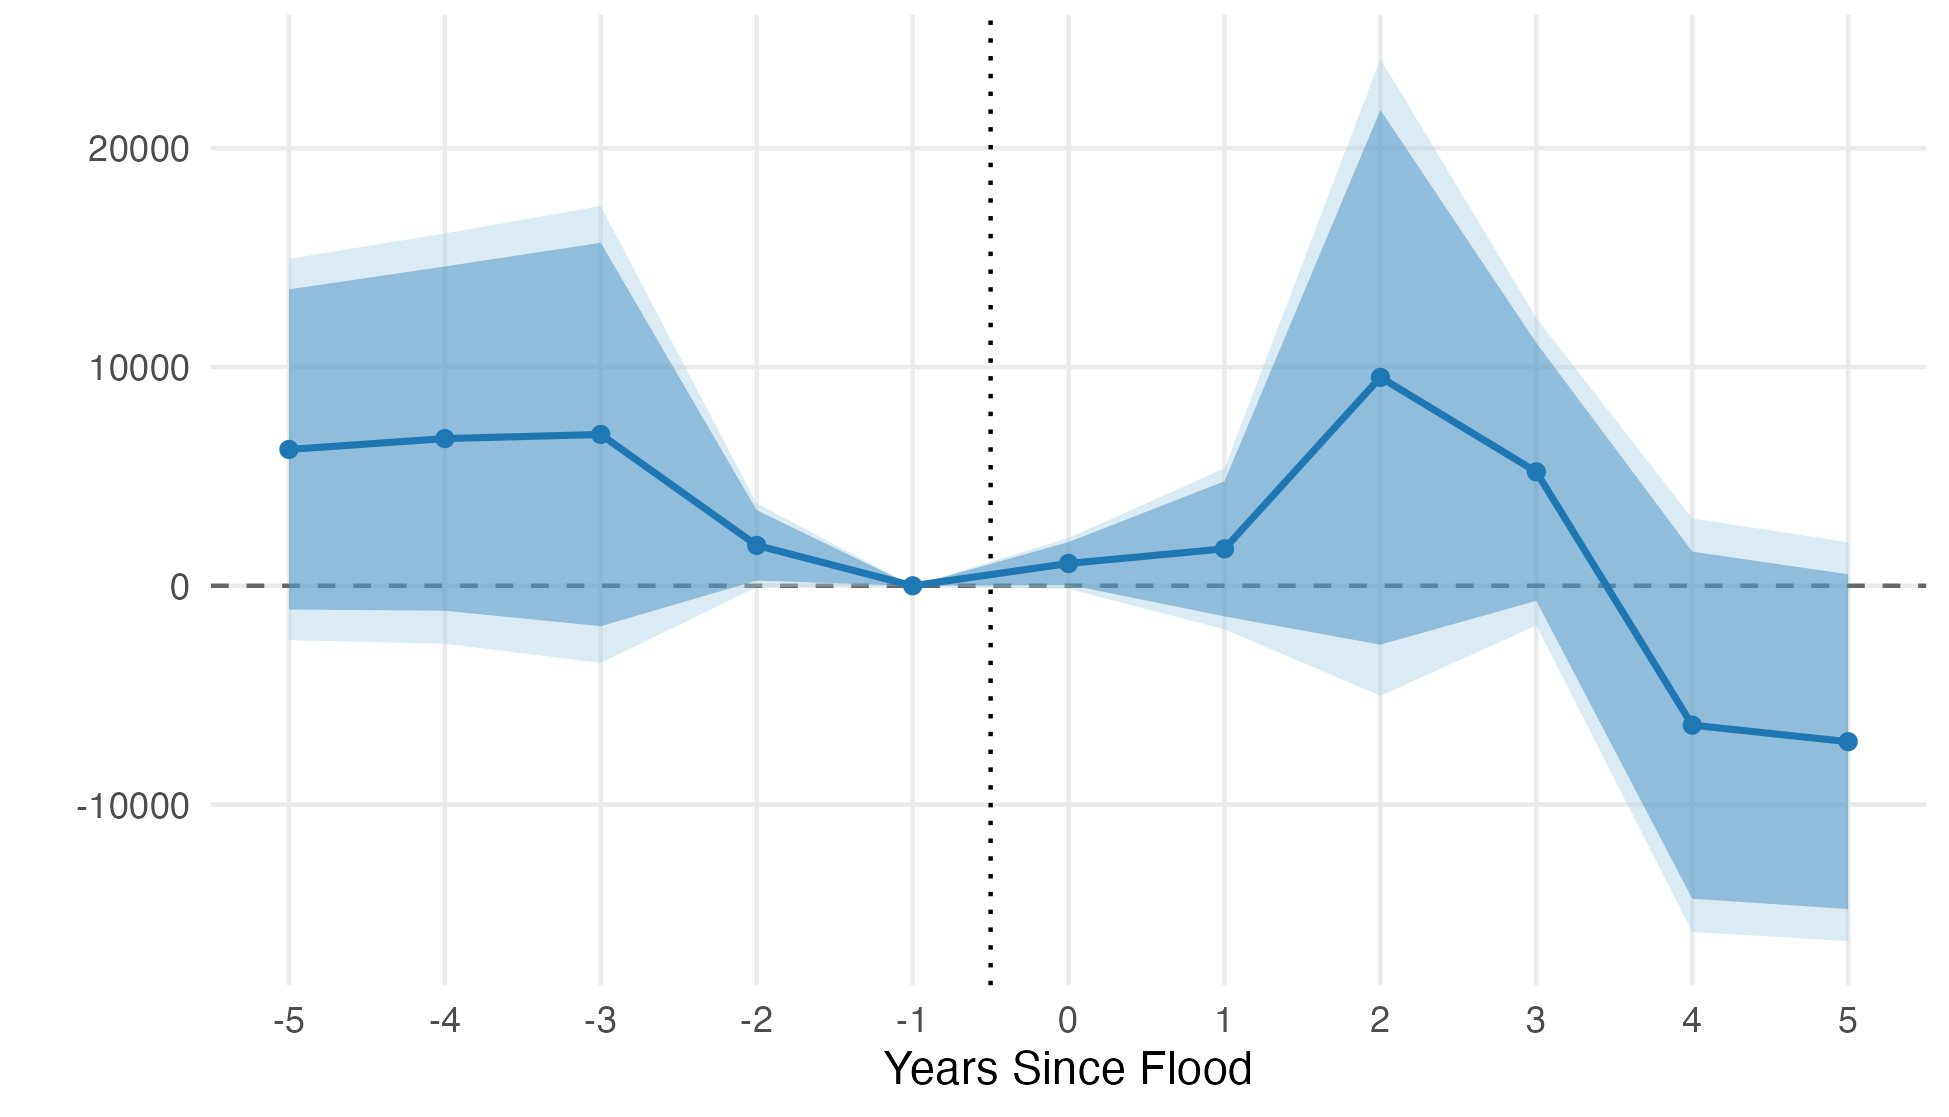
\includegraphics[width=\linewidth]{figures/Results/Analysis_Communes/IRF_CAPISOC_SIRET_pooled.png}
    \subcaption{Share capital}
    \label{}
  \end{subfigure}
  \begin{subfigure}[b]{0.32\textwidth}
    \centering
    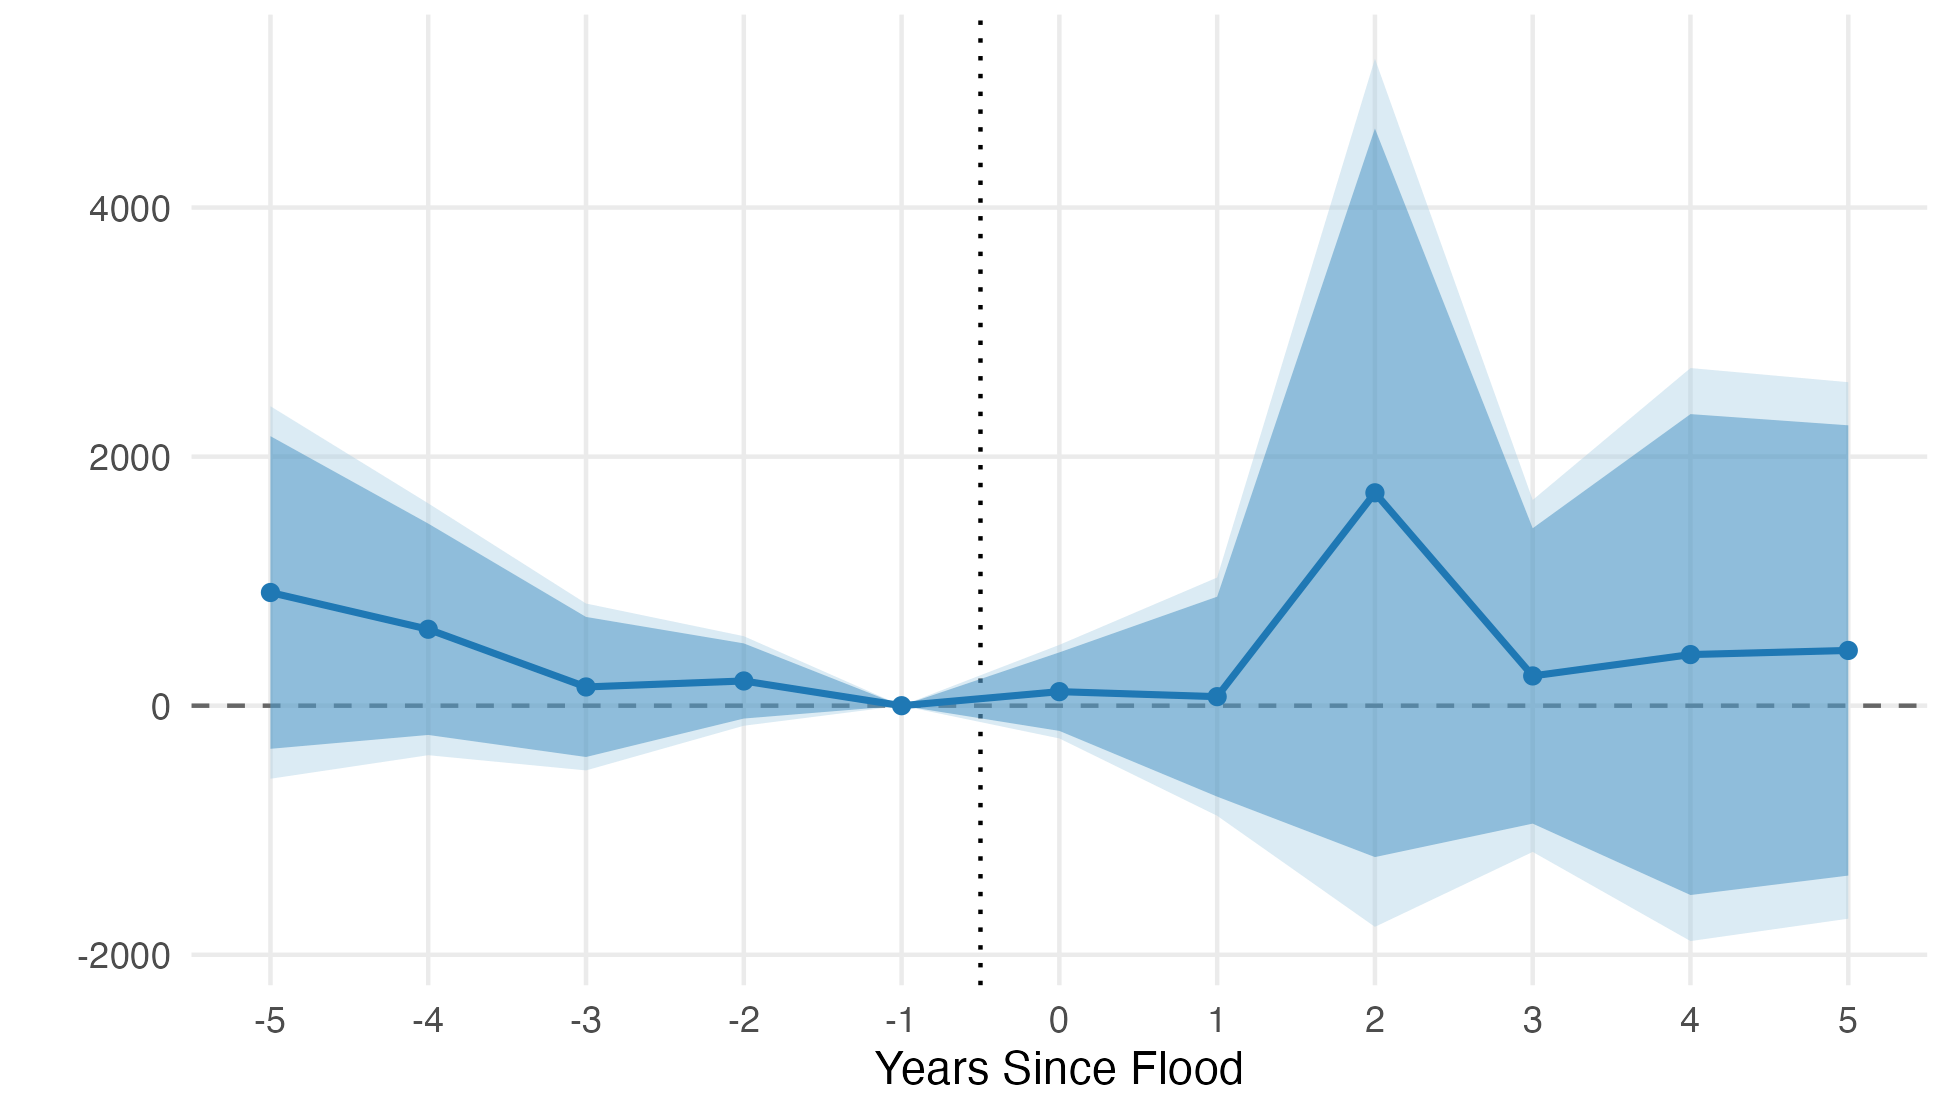
\includegraphics[width=\linewidth]{figures/Results/Analysis_Communes/IRF_b319_SIRET_pooled.png}
    \subcaption{Current profit before tax}
    \label{}
  \end{subfigure}


\end{figure}

%%%%%%%%%%%%%%%%%%%%%%%%%%%%%%%
\begin{figure}[htbp]
  \centering
  \caption{\textbf{Figure \ref{fig:IRF_litorale_comparison}:} Flood impacts by coastal exposure (litorale)}
  \label{fig:IRF_litorale_comparison}
  
    \begin{subfigure}[b]{0.45\textwidth}
    \centering
    \textbf{Litorale = 0}
  \end{subfigure}
  \hspace{1em}
  \begin{subfigure}[b]{0.45\textwidth}
    \centering
    \textbf{Litorale = 1}
  \end{subfigure}

  \vspace{0.8em}
  
  % Row 1: EFF3112
  \begin{subfigure}[b]{\textwidth}
    \centering
    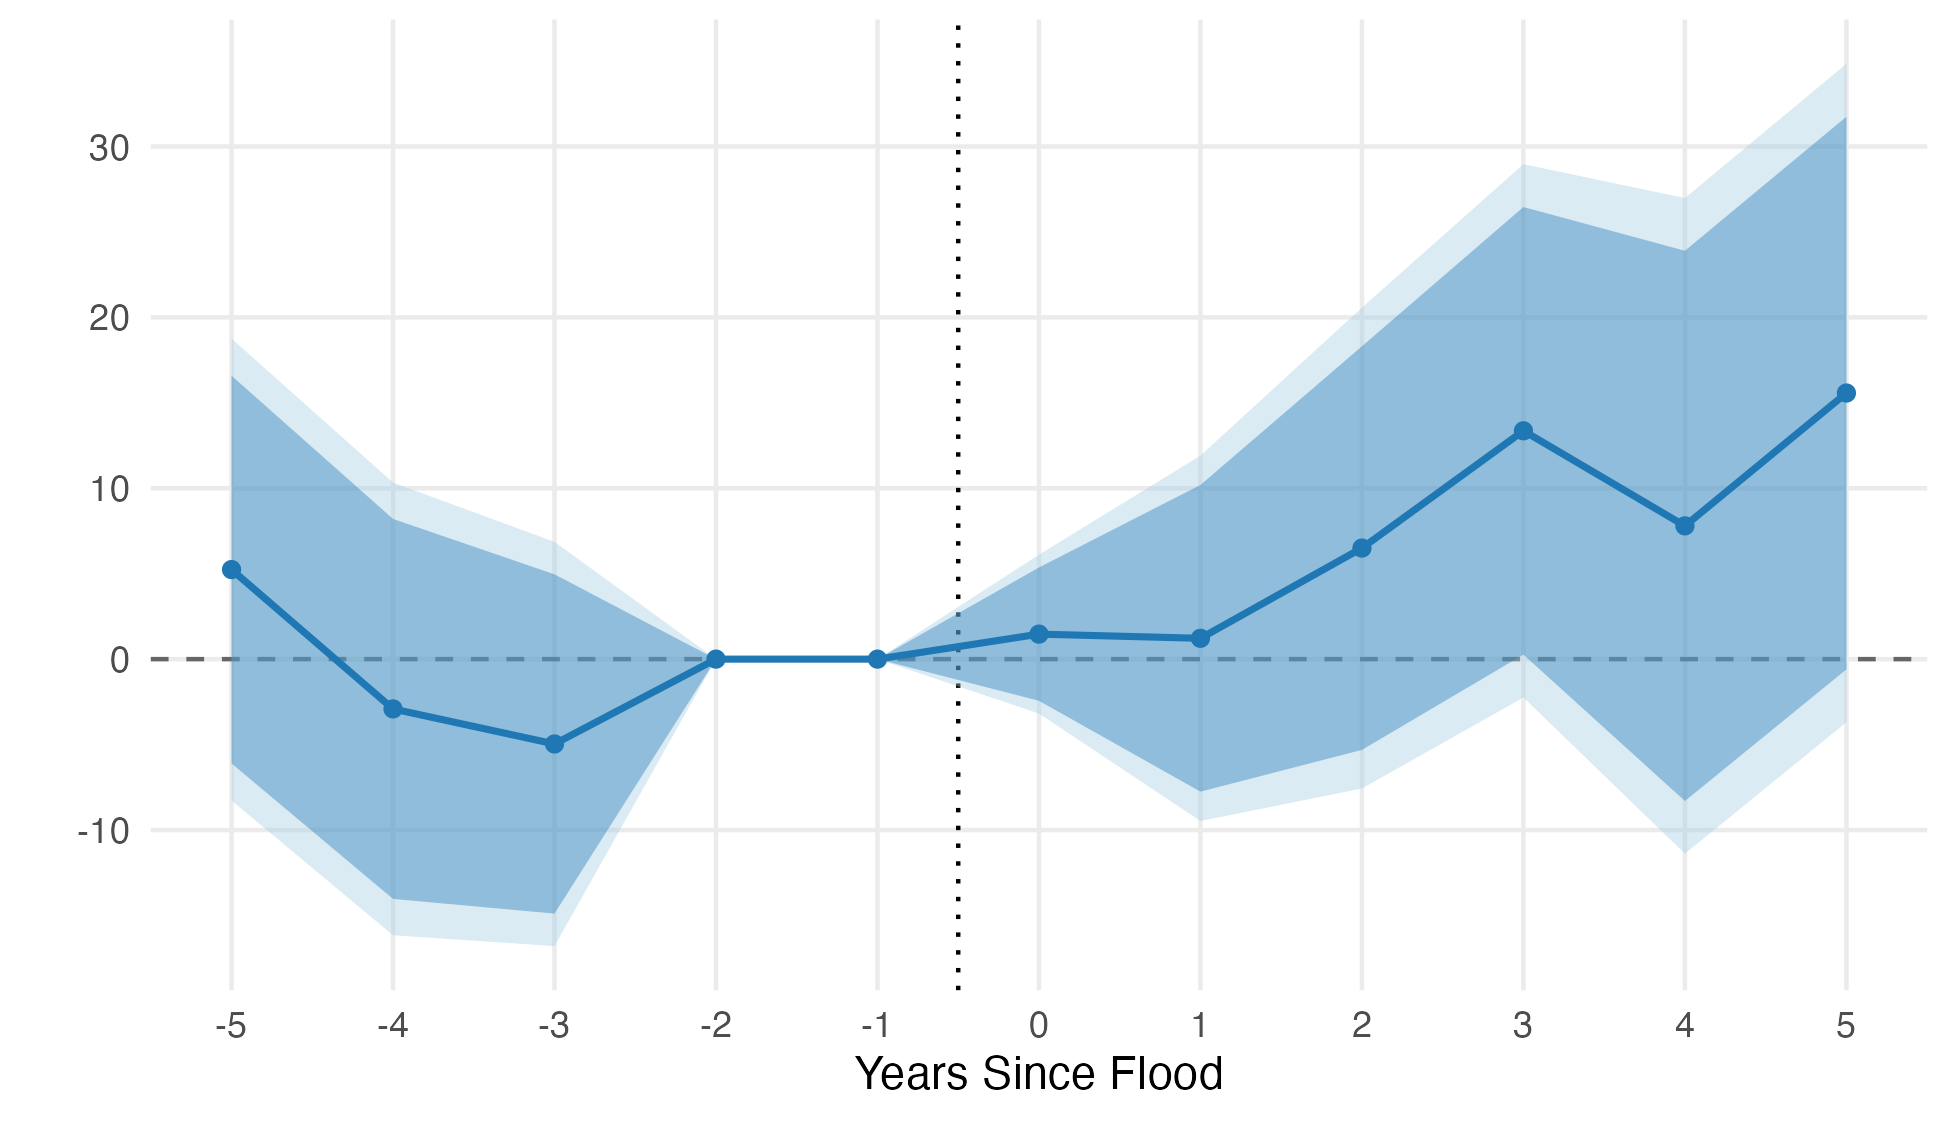
\includegraphics[width=0.45\textwidth]{figures/Results/Analysis_Communes/litorale/IRF_EFF_3112_litorale_0.png}
    \hspace{1em}
    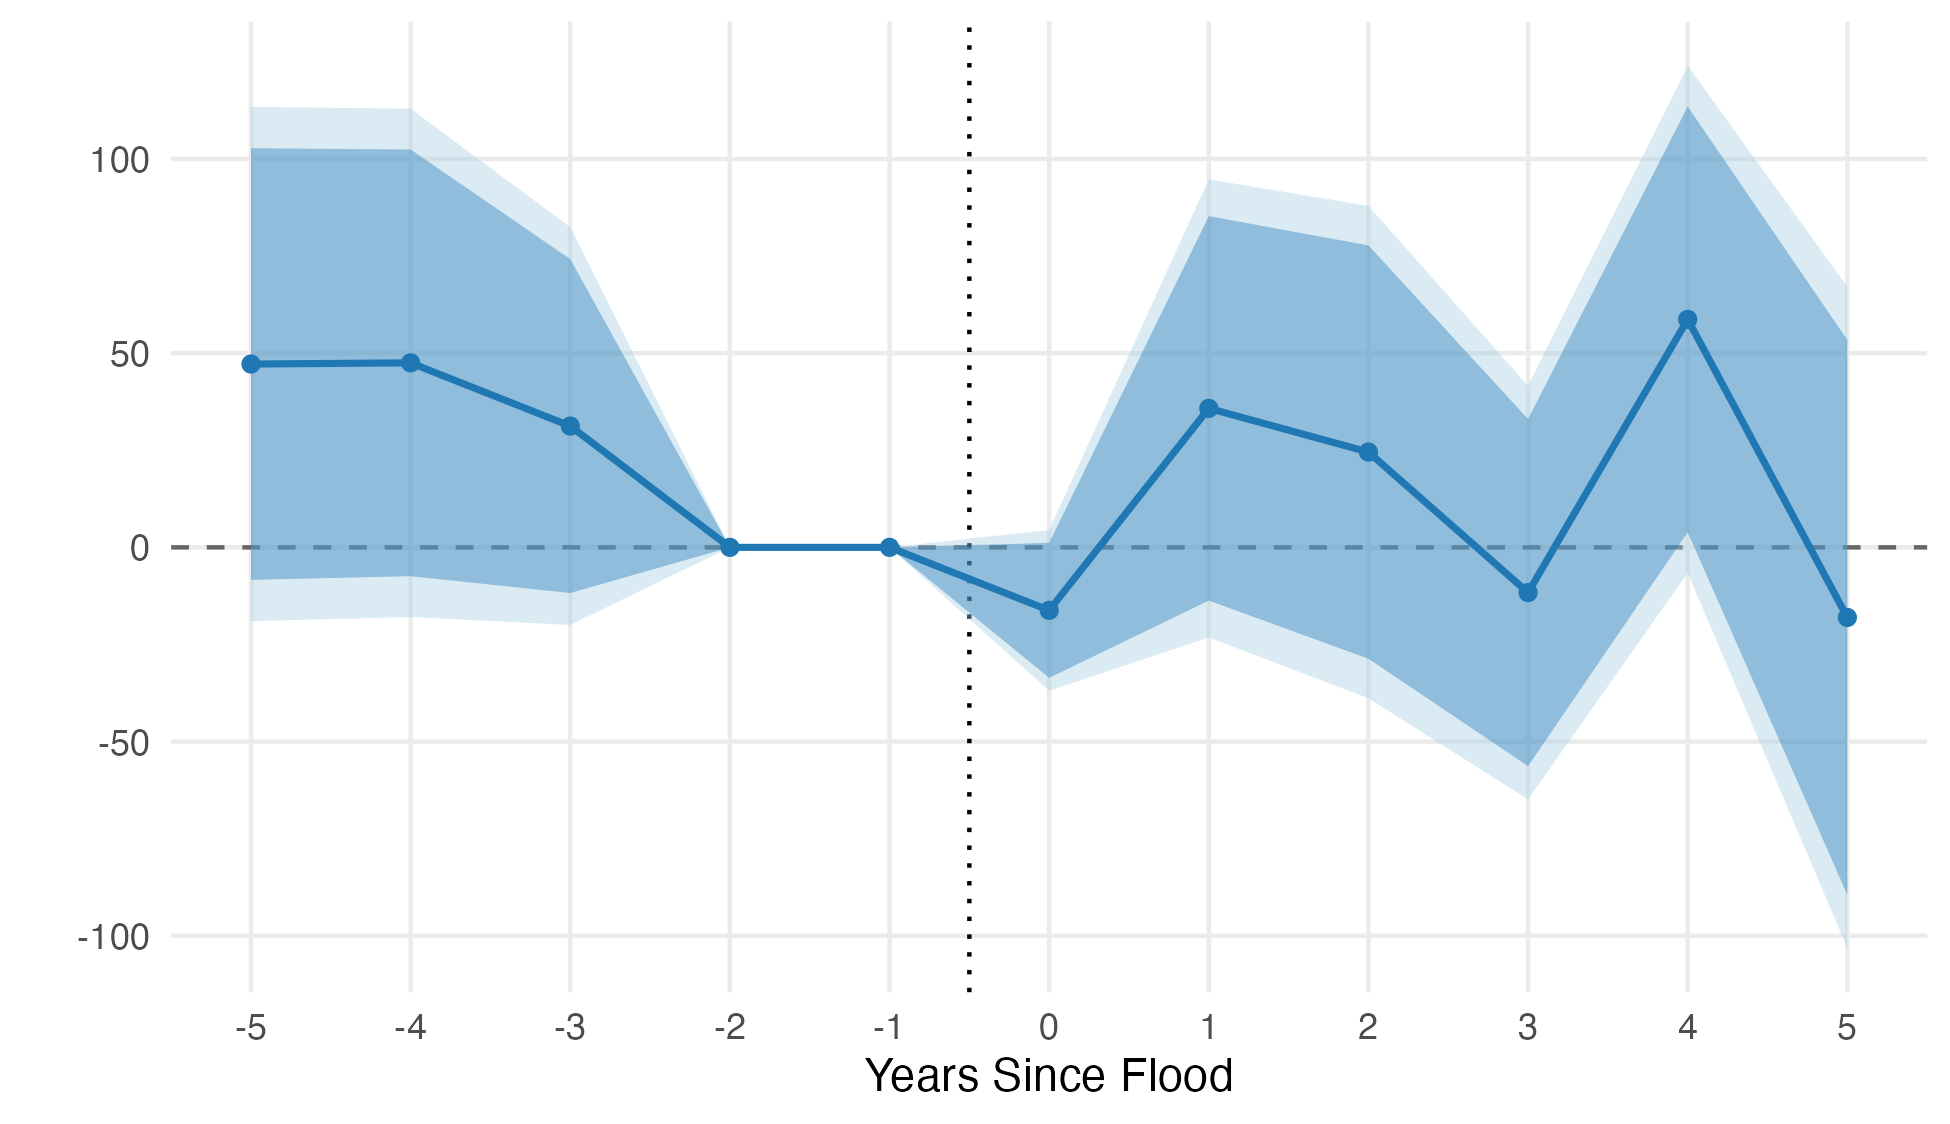
\includegraphics[width=0.45\textwidth]{figures/Results/Analysis_Communes/litorale/IRF_EFF_3112_litorale_1.png}
    \subcaption{Headcount at 31.12}
  \end{subfigure}

  \vspace{1.2em}

  % Row 2: AVGWAGE3112
  \begin{subfigure}[b]{\textwidth}
    \centering
    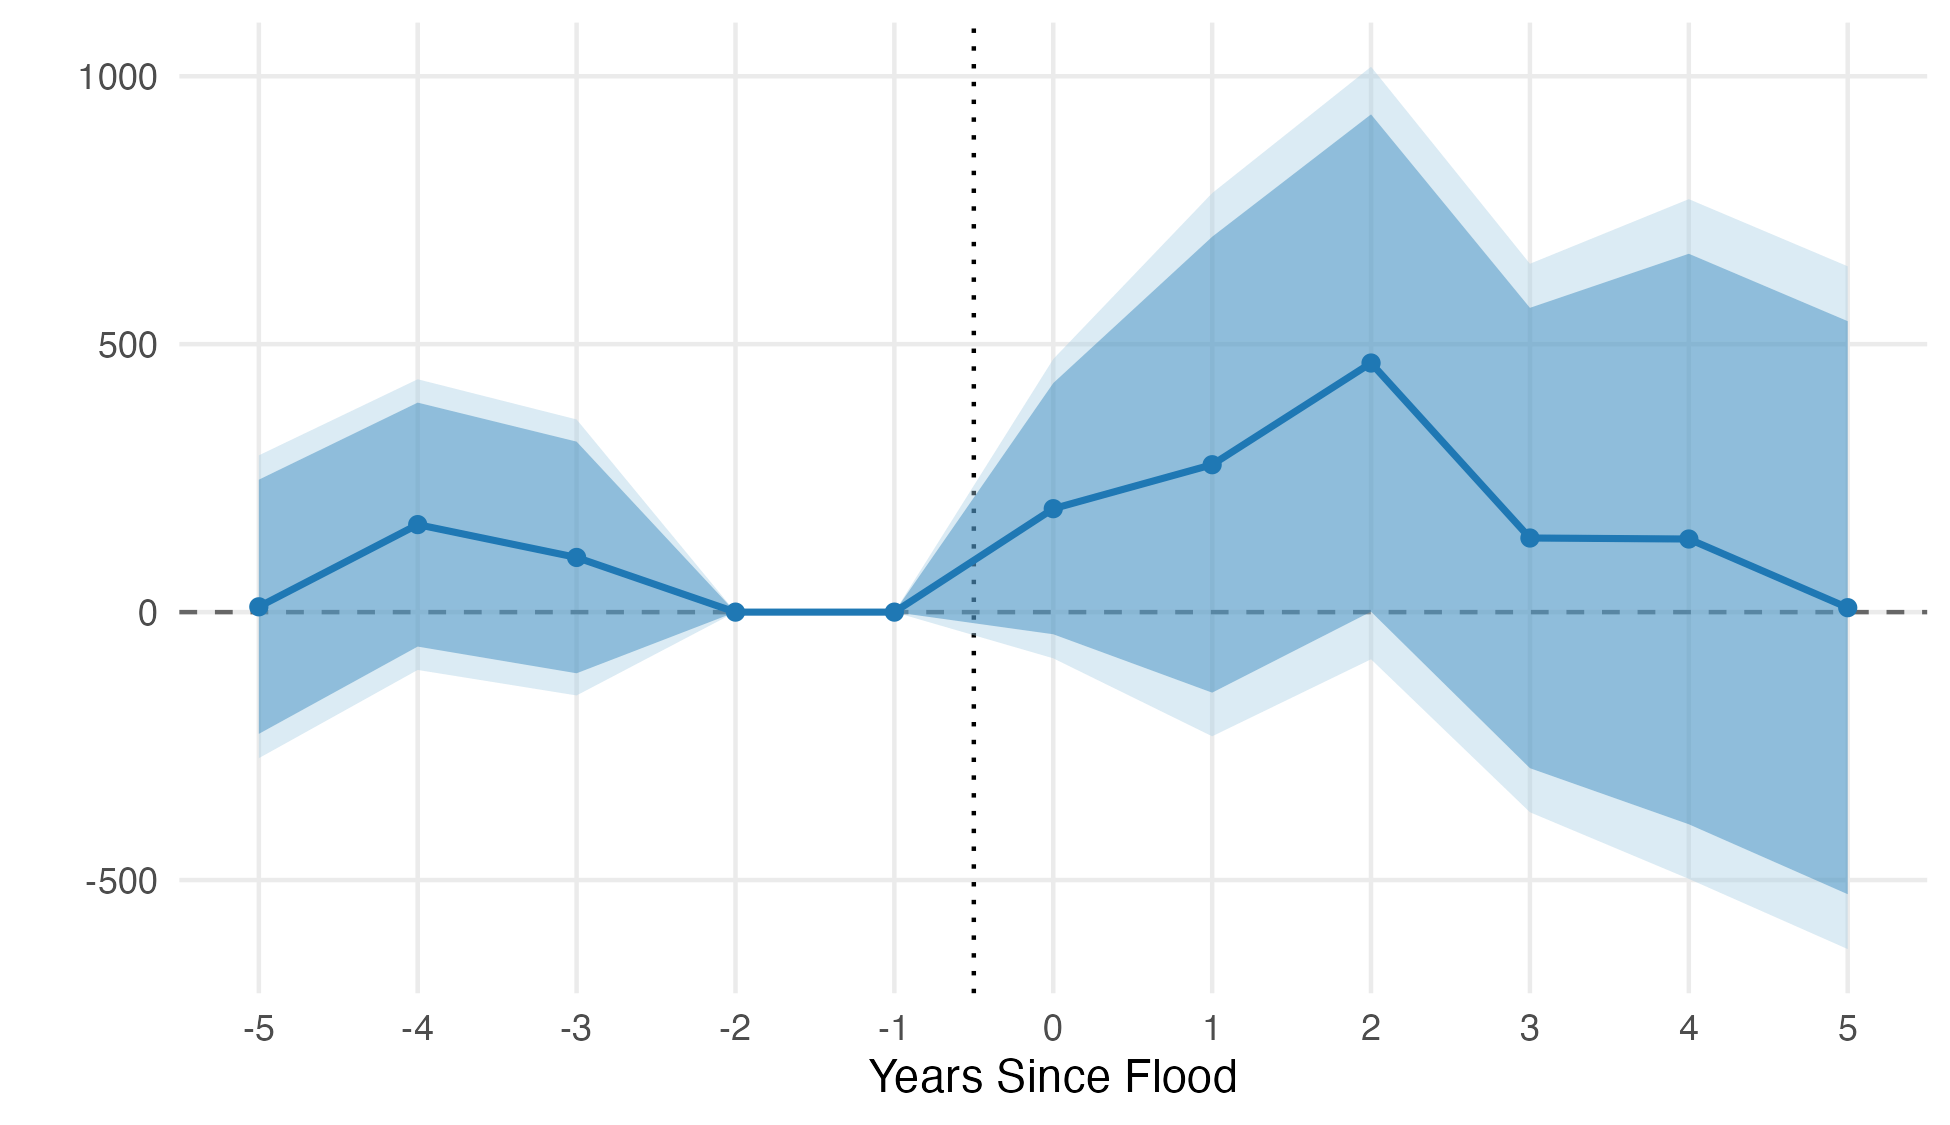
\includegraphics[width=0.45\textwidth]{figures/Results/Analysis_Communes/litorale/IRF_AVGWAGE_litorale_0.png}
    \hspace{1em}
    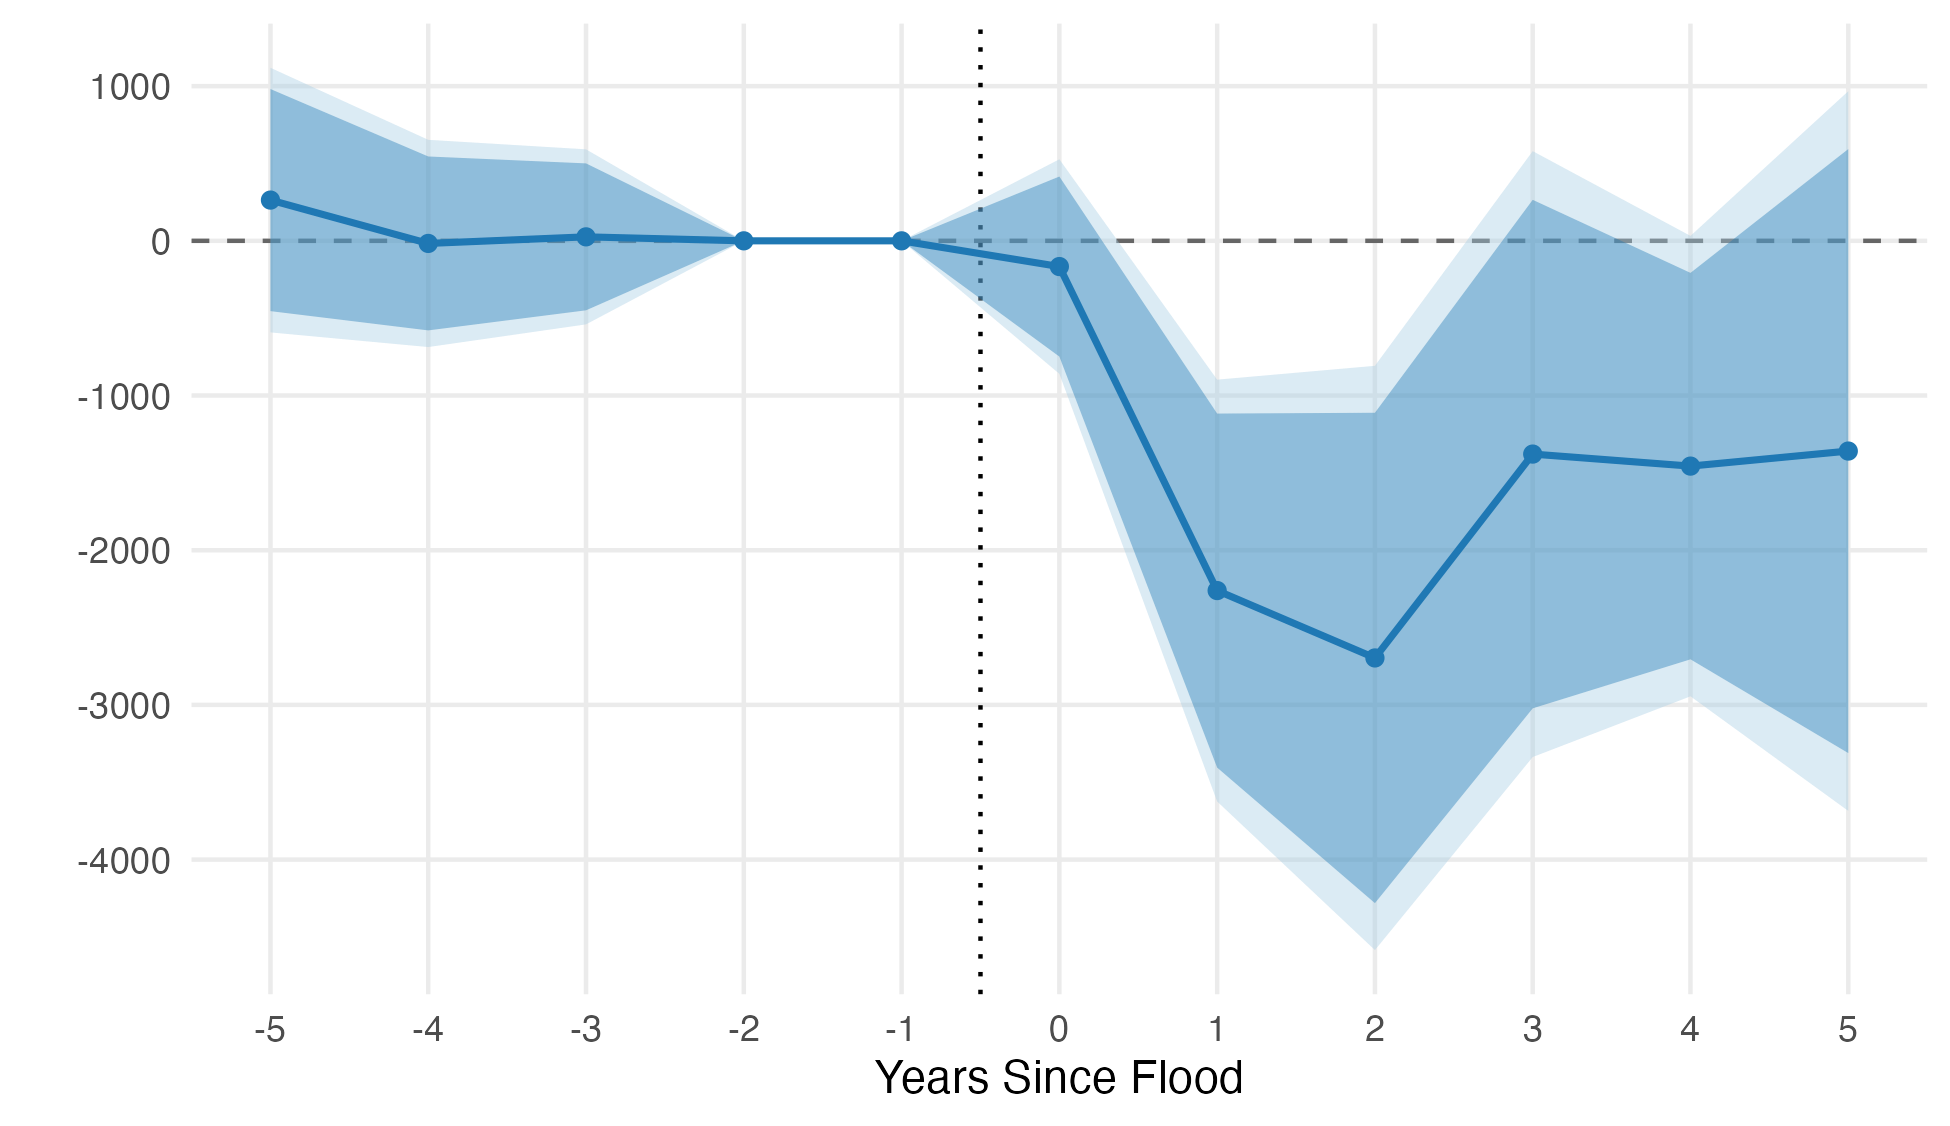
\includegraphics[width=0.45\textwidth]{figures/Results/Analysis_Communes/litorale/IRF_AVGWAGE_litorale_1.png}
    \subcaption{Wages at 31.12}
  \end{subfigure}

  \vspace{1.2em}

  % Row 3: Revenue
  \begin{subfigure}[b]{\textwidth}
    \centering
    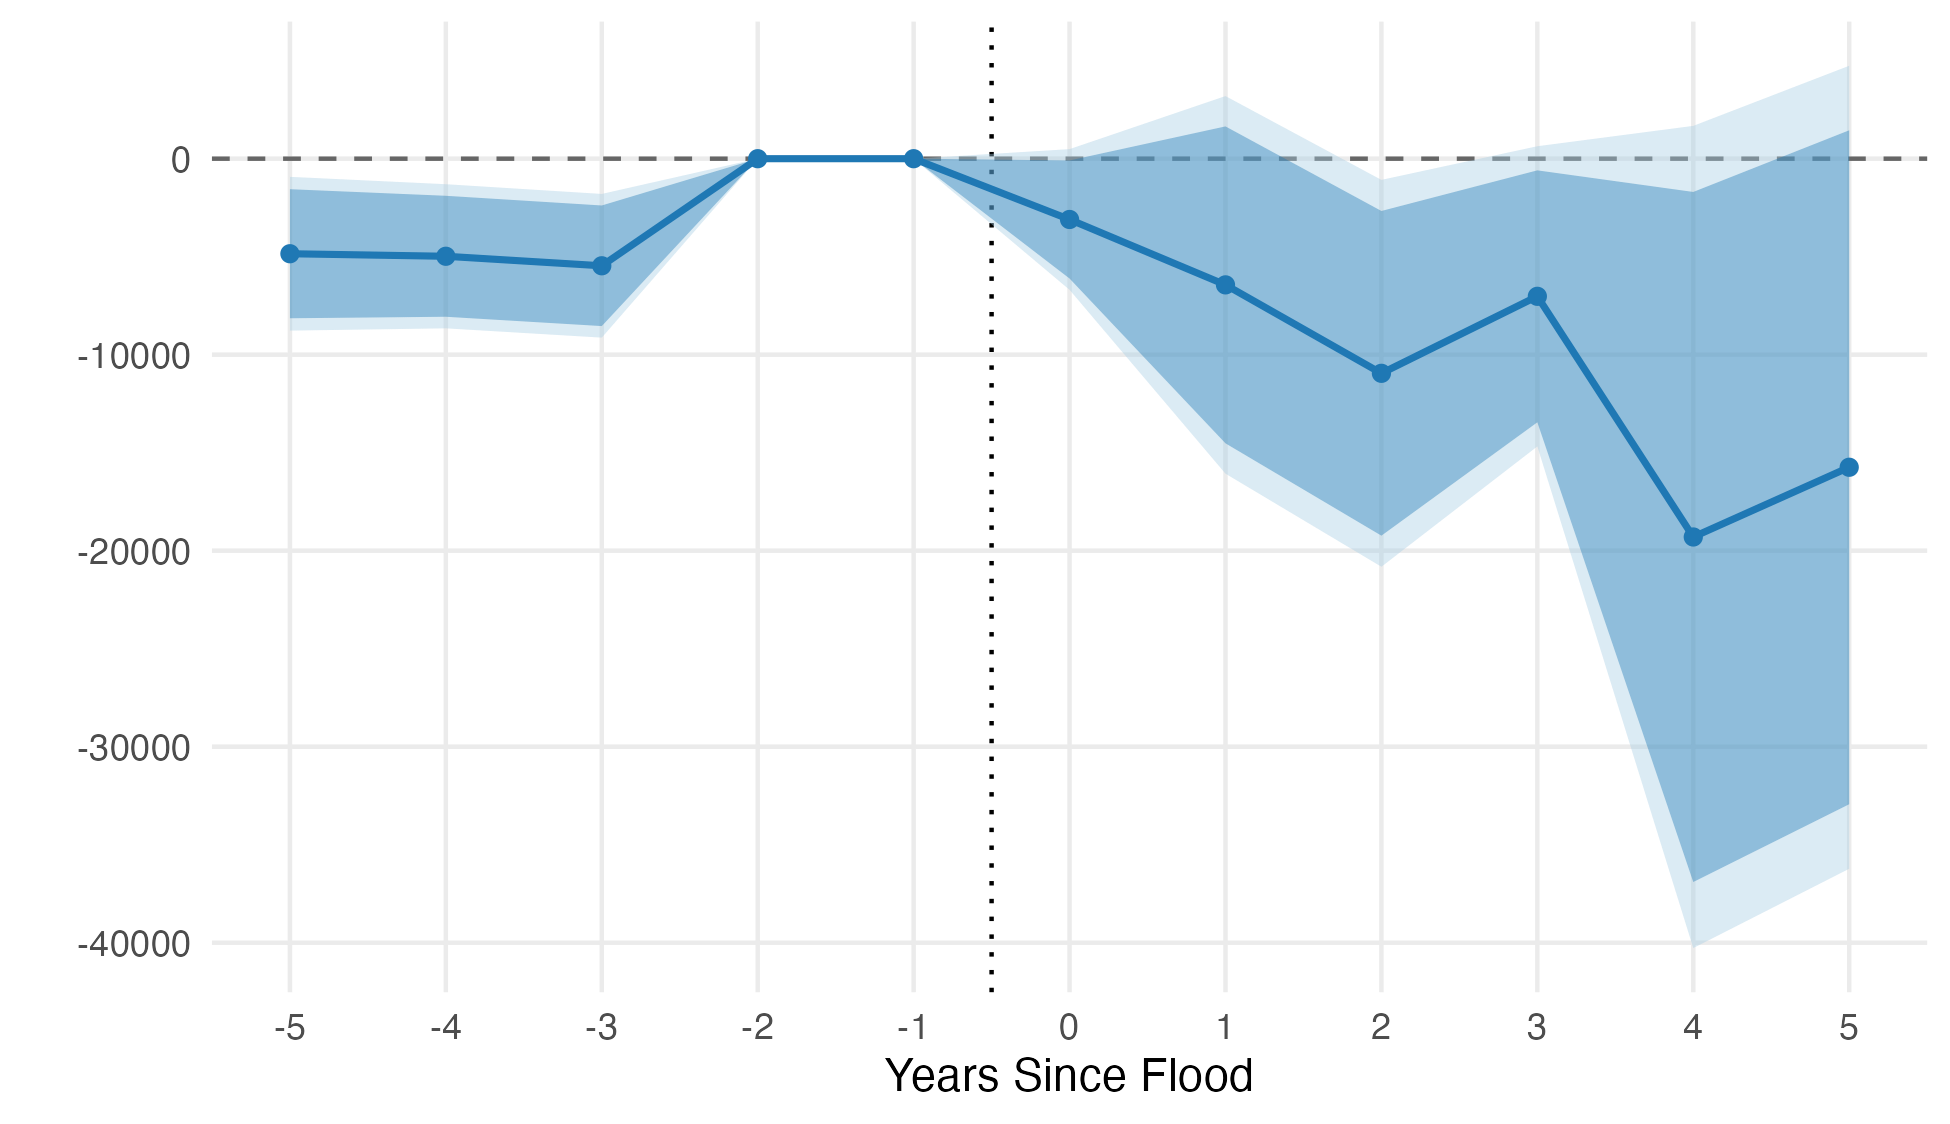
\includegraphics[width=0.45\textwidth]{figures/Results/Analysis_Communes/litorale/IRF_redi_r310_SIRET_litorale_0.png}
    \hspace{1em}
    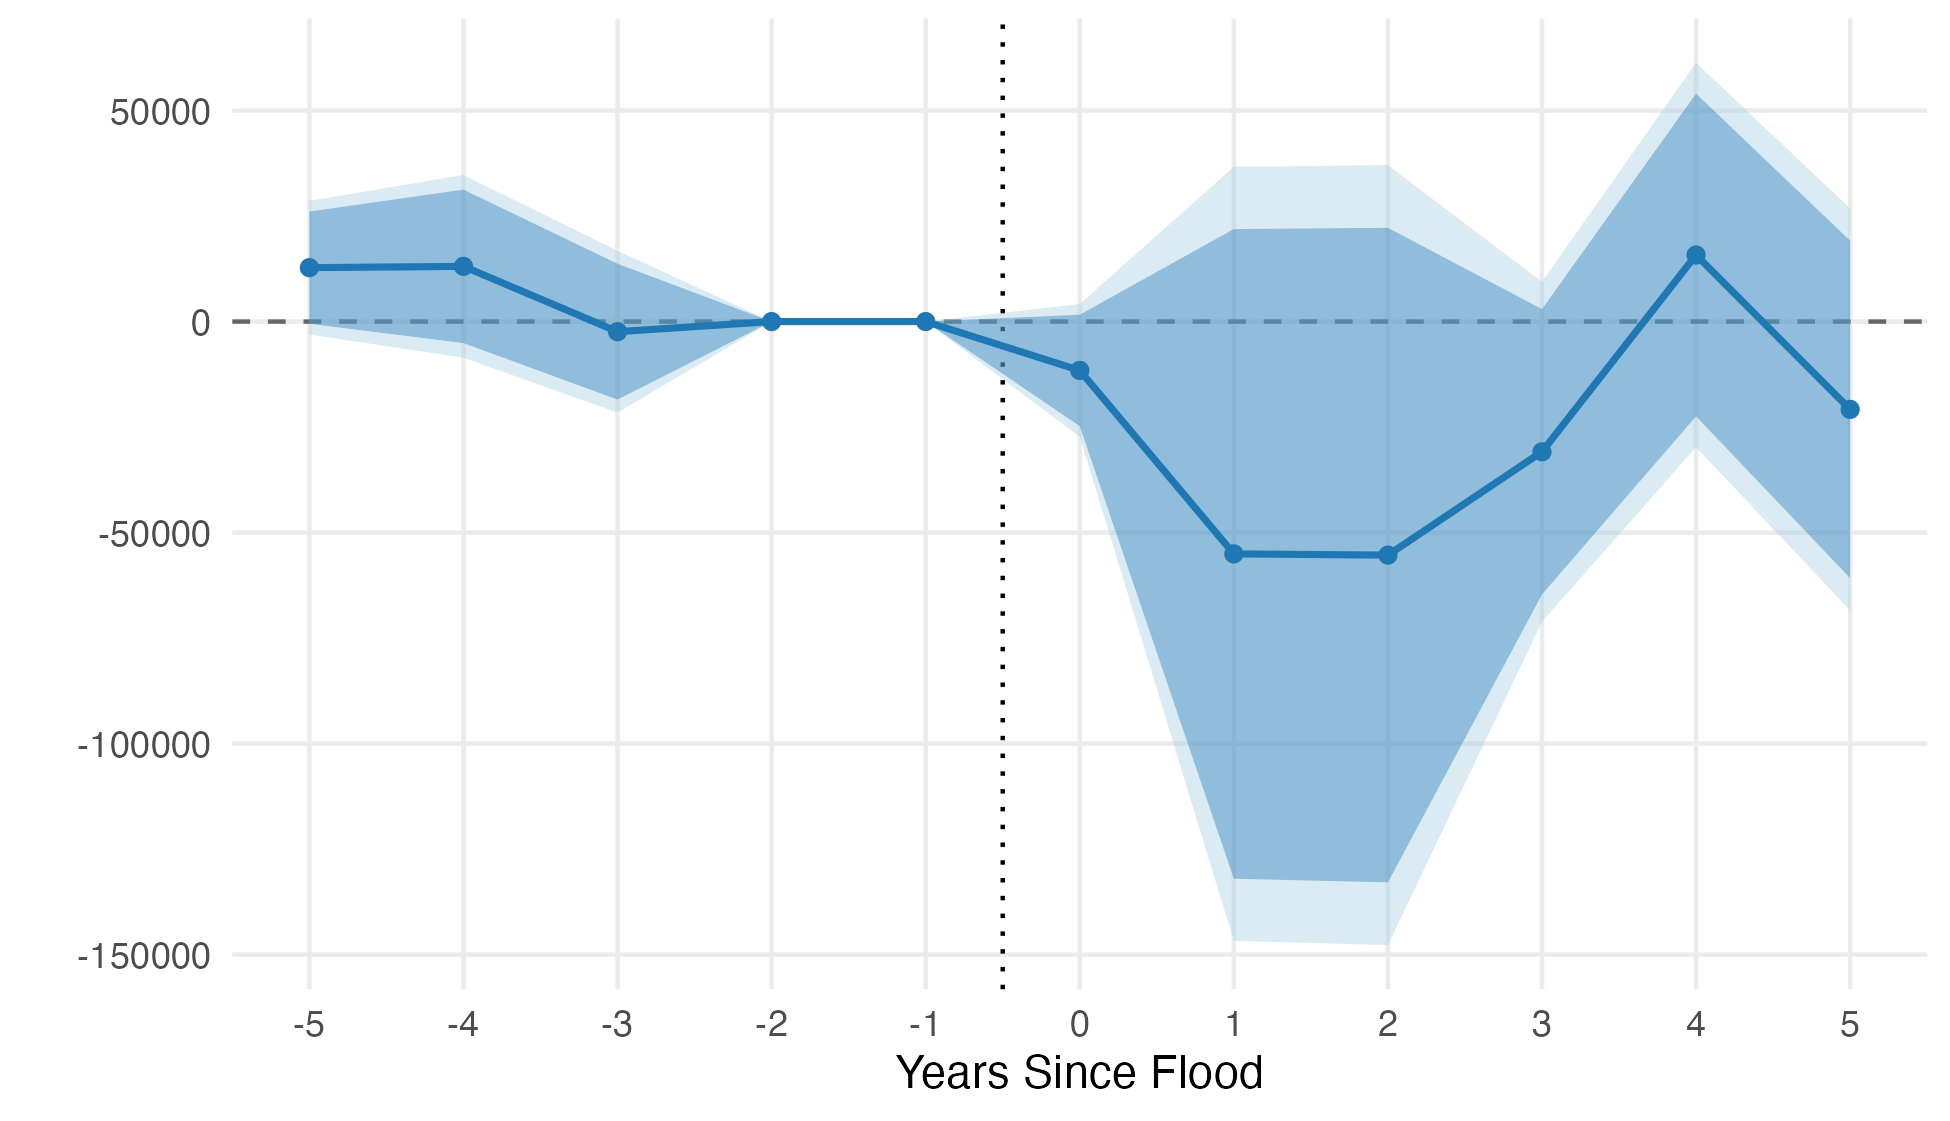
\includegraphics[width=0.45\textwidth]{figures/Results/Analysis_Communes/litorale/IRF_redi_r310_SIRET_litorale_1.png}
    \subcaption{Total Revenue}
  \end{subfigure}
   \caption*{\raggedright\textit{Note}:  Shaded areas indicate 90\% and 95\% confidence intervals. The first flood for a commune is defined as the first year in which the commune witnessed a \textit{CatNat} flooding episode in the sample. Since the outcomes data starts in 2010 but the floods can be tracked since 1985, only those communes that did not witness any flood event in the period 2000-2009 are included in the analysis. To get to the aggregate variables from establishment-level information, the variables are then summed across communes for each year using labor share weights.}
\end{figure}

To examine heterogeneity, I stratify communes by coastal exposure. Figure \ref{fig:IRF_litorale_comparison} shows that coastal communes experience somewhat larger short-term declines in revenues and wages following floods, whereas non-coastal communes exhibit flatter trajectories. The confidence intervals remain wide, so these patterns should be interpreted with caution. Still, the comparison suggests that exposure to the sea amplifies short-run damages, consistent with physical vulnerability and higher baseline flood risk in coastal areas.\\

This designation of a flooding episode is place-based, tied to the specific communes affected, and primarily triggers compulsory insurance coverage for damages sustained. It does not automatically unlock substantial public funding for infrastructure reconstruction or direct fiscal transfers to households and firms. Nevertheless, it ensures regulated insurance payouts, offering financial relief to those affected. \cite{indaco2021hurricanes} find a similar mechanism at work in the U.S. hurricane context, where insured losses are quickly compensated but public transfers play only a minor role.
Other mechanisms may also explain why aggregate effects appear muted. First, CCR insurance payouts cushion establishment-level losses and provide immediate liquidity, preventing wider economic dislocation. Second, firm entry and exit dynamics can rebalance local activity, with new entrants or expanding firms offsetting losses from those directly affected. Third, labor mobility between communes of work and residence helps smooth employment adjustments, as workers can shift jobs or commute elsewhere even if their local establishment is disrupted. Fourth, land use and cementification patterns condition how economic activity is exposed to flooding, with more built-up areas often facing higher direct damages but also faster recovery due to greater infrastructure and capital intensity. Finally, labor market regulation and unemployment insurance shape how shocks are absorbed: where firing costs are high, firms may adjust via capital rather than layoffs, while workers benefit from income smoothing through insurance or temporary withdrawal from the labor force.

These findings fit into a broader empirical pattern. \cite{roth2020local} shows that in U.S. counties, unlike hurricanes and tornadoes, floods tend to have a significant negative effect on US counties only in the year of the disaster, followed by a modest positive effect in the medium term, suggesting that aggregate recovery is rapid. \cite{bilal2023anticipating} emphasize that anticipation of climate risks influences location and investment decisions in the U.S., so observed damages may already reflect selection out of the most vulnerable areas. \cite{fatica2024floods} find that in Europe, financial resilience is shaped by insurance institutions and fiscal frameworks, which buffer aggregate outcomes even when establishment-level shocks are severe. Taken together, the evidence indicates that while establishments experience significant disruptions from floods, commune-level aggregates show limited persistent effects, reflecting the role of insurance, reallocation, and recovery mechanisms in attenuating shocks at higher levels of aggregation.

% \textbf{Mechanisms:}
% \begin{itemize}
%     \item CCR payouts
%     \item Firm entry and exit
%     \item perceived flood risk drives selection
%     \item commune of work vs residence: do people still work there or
%     \item Level of cementtifiaction; economic activity like VA is linked to flooding confounders
%     \item Long term scarring of flooding? Labour regulation and (un)employment insurance determine strenght of adjustment mechanisms of workeers and firms. If strong regulation, firms can't fire then adjust in capital. Workers, can switch job if wages go down. Or, workers can adjust by stopping work and training! 
%     \item Cost discoverty
%     \item: 
%     \end{itemize}




% \textbf{Comparison with other effects in the literature:}
% \begin{itemize}
%     \item in \cite{roth2020local}, unlike for other hazards such as hurricane and tornadoes, floods have a significant negative effect on US counties only in the year of the disaster, followed by a modest positive effect in the medium term.  why can't see in financial variablels maybe
%     \item Bilal (anticipating climate chang ein the US)
%     \item Fatica et al (vulnerabilities and resilience to natural disasters in Europe)

%     \item Similar to what other shocks, how can one model these macro done in Bilal, but otherr exapmles if structural models now.
% \end{itemize}


% Read 7 Discussion in Wing stacked, and compare to Dube. I want to talk about ATT and waht exactly I am targeting as estimand.


% Possible Robustness Checks:

% \begin{itemize}

%     \item Vary slightly Flood Risk Index taking into account variation in depth of water in order to categorize chronically exposed areas vs. areas prone to rare but intense flooding
%     \item Sample of mono-establishments only
%     \item include all floods and not only extreme ones
%     \item The spatial scale at which commuting and supply-chain spill-overs are most salient is important, i would like to estimate at ZEMPT level. 
% \end{itemize}
